\documentclass[../main]{subfiles}
\begin{document}
\chapter{枝の増減に伴う同期状態の変化}
\label{chap:method-3body}
\section{問題設定及び数値実験}
\label{sec:method-3body-settting}
振動子ネットワークのふるまいを調べる際は,ネットワークの構造と振動数分布を定める必要がある.

ネットワークの構造としては,最も単純でありながら多様な性質をもつErd\H{o}s–R\'{e}nyi model(ERモデル)$\Gamma_{n,m}$ を用いる.
そして,枝の本数$m$を変化させることでモデルの構造を変化させることで振動子ネットワークのダイナミクスを変化させる.
すなわち,$n$ 体の振動子ネットワークにおいて枝をランダムに選択し追加・削除を行うことで,$m=0$から$m=n(n-1)/2$まで枝の本数を連続的に変化させる.
このとき,構造の変化に伴い同期状態が変化することが考えられる.

固有振動数の分布として,一般にはローレンツ分布などの連続分布\cite{kuramoto1975}から二項分布のような離散分布\cite{1992BonillaNeuSpigler}まで考えられる.
本論文では,異なる固有振動数を持つ振動子の同期を扱う最も簡単な分布としてニ項分布を用いる.
特に,一般性を失わず$\pm 1$の二項分布$\operatorname{Bin}(n,p)$を用いる.

よって,ネットワークの各振動子の位相$\phi_i$($i=1,2,\ldots,N$)は,以下のような方程式に従う.
\begin{equation}
    \dot{\phi}_i=\omega_i+\lambda\sum_{j=1}^n A_{ij}\sin(\phi_j-\phi_i)
\end{equation}
ただし,振動子$i$の固有振動数$\omega_i$は確率$p$で$1$,確率$1-p$で$-1$をとる確率変数である.
ここで,全ての振動子が結合している状況以外も考慮するために式\eqref{eq:kuramoto-network}とは異なり,結合強度を振動子の数でスケーリングせず$\lambda$としていることに注意せよ.

$n=6$での数値実験の結果を図\ref{fig:cutting_N6K1}に示す.
ただし,時刻$t\ (0\leq t\leq T)$で位相$\phi_i(t)$の node $i$の実効振動数は,$\Omega_i^{\mathrm{eff}}\coloneqq(\phi_i(T)-\phi_i(T/2))/(T/2)$で定めた.
ここで,$m=5$における node $1$のように,枝の増加により増加前に同期していた node と非同期になり別の node と同期する,つまり同期クラスタが変化する現象が見られる.
以下,このような同期状態の変化を「鞍替え」と呼ぶこととする.
この鞍替え現象は,振動子が鎖状に繋がりの隣接した振動子の一方からのみ相互作用を受ける蔵本モデルにおいて結合強度を全て同じ値で変化させた場合に発生することが知られている\cite{XiaHuang:130506}(付録参照).
しかしながら,ネットワーク構造の変化で発生することは知られておらず,
疎なネットワークにおける微視的なクラスタリングパターンの理解において重要な役割を果たすと考えられる.
また,ネットワーク全体のクラスタリングパターンの変化は,一部の振動子についての同期現象と鞍替え現象に分割して理解することができる.

次節ではこの鞍替え現象に注目し解析を行う.

\begin{figure}[tbp]
\centering
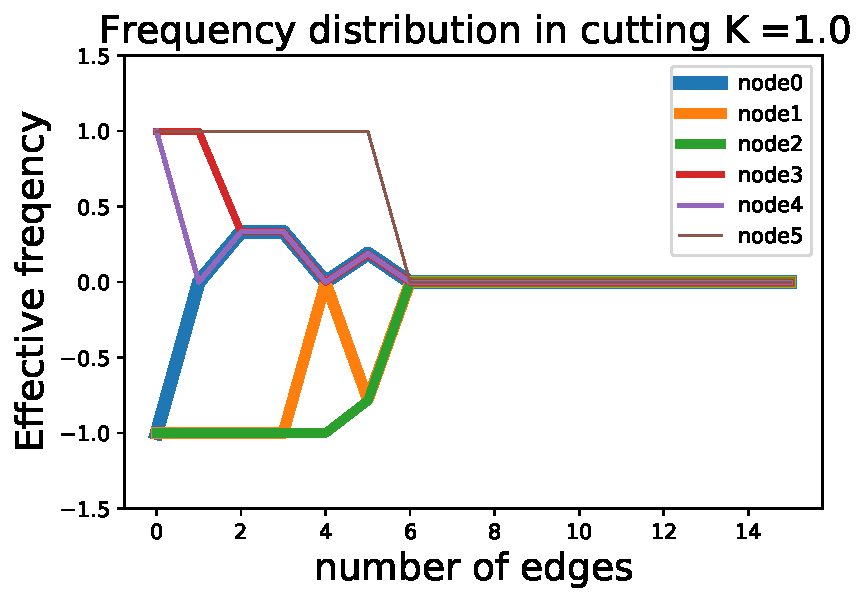
\includegraphics[width=105mm]{./images/cutting_N6K10.pdf}
\centering
\caption{固有振動数$1$の振動子3つと固有振動数の$-1$の振動子3つからなる6体の振動子ネットワークにおいて,枝を1本ずつランダムに選び全接続まで連続的に増やしたときの各振動子の実効振動数の変化を表す.ただし$\lambda=1.0$である.
$m=5$における node $1$では,枝の増加により増加前に同期していたnodeと非同期になり別のnodeと同期する「鞍替え」が見られる.}
\label{fig:cutting_N6K1}
\end{figure}

\section{鞍替え現象のモデル化}
ある$L$体の集団が$M$体の集団から$N$体の別の集団に鞍替えを起こすとき,以下のようにモデル化できる.
\begin{screen}
実効振動数$\omega_L$の$L$体の振動子集団$\Omega_L$が実効振動数$\omega_M$の$M$体の振動子集団$\Omega_M$との間に$m$本の枝で繋がっており,また,実効振動数$\omega_N$の$N$体の振動子集団$\Omega_N$との間に$n$本の枝で繋がっている.
ただし,振動子集団$\Omega_M$と振動子集団$\Omega_N$との間に枝は存在しないとする.(図\ref{fig:switch})\\
枝の本数$m,n$が変化すると,振動子の実効振動数が変化し同期状態が変化する.
\end{screen}

\begin{figure}[tbp]
\centering
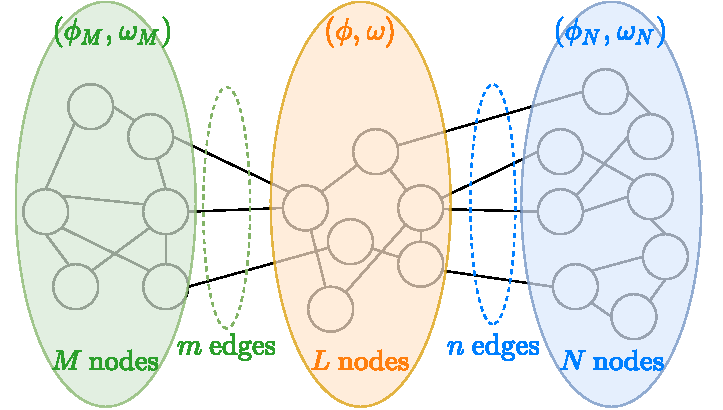
\includegraphics[width=105mm]{./images/three_obj_before.pdf}
\centering
\caption{鞍替え現象に関わる部分ネットワーク}
\label{fig:switch}
\end{figure}

% このとき,$\Omega_M\ (\Omega_N)$に属する振動子間の枝の本数が$m\ (n)$と比べ十分多いと仮定する.
このとき,集団間の枝を削除したとき,それぞれの振動子集団に属する振動子同士が同期することを仮定する.
すると,それぞれの振動数集団に属する振動子がそれぞれ同一の位相・固有振動数を持つとして平均場近似を行うことができ,発展方程式は以下のようになる.
\begin{align}
    \label{eq:3body-default}
    \begin{split}
        \dot{\phi_L}&=\omega_L+\frac{n}{L}\lambda\sin\left( \phi_N-\phi_L \right)+\frac{m}{L}\lambda\sin\left( \phi_M-\phi_L \right),\\
        \dot{\phi}_M&=\omega_M+\frac{m}{M}\lambda\sin\left( \phi_L-\phi_M \right), \\
        \dot{\phi}_N&=\omega_N+\frac{n}{N}\lambda\sin\left( \phi_L-\phi_N \right).    
    \end{split}
\end{align}
特に,結合強度を$K=n\lambda$で定義し直し,結合強度比$a=m/n,\ L=1,\ M=1,\ N=1$と仮定すると,図\ref{fig:3body}のような鞍替えする振動子を中央とする鎖状の3体ネットワークに簡略化される.

\begin{figure}[tbp]
    \centering
    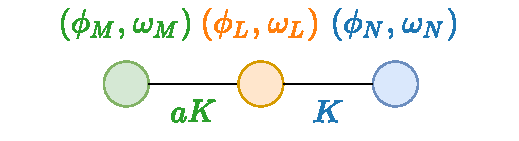
\includegraphics[width=105mm]{./images/three_obj_after.pdf}
    \centering
    \caption{鞍替え現象に関わる部分ネットワークを簡略化した鎖状の3体ネットワーク}
    \label{fig:3body}
\end{figure}

\begin{align}
    \label{eq:3body}
    \begin{split}
        \dot{\phi}_L&=\omega_L+K\sin\left( \phi_N-\phi_L \right)+aK\sin\left( \phi_M-\phi_L \right),\\
        \dot{\phi}_M&=\omega_M+aK\sin\left( \phi_L-\phi_M \right), \\
        \dot{\phi}_N&=\omega_N+K\sin\left( \phi_L-\phi_N \right).    
    \end{split}
\end{align}
3体系においてパラメータを変化させることで2体の同期に関わる鞍替え現象を観測できることが予想されると同時に,3体全体の同期現象を調べることもできる.
ネットワーク全体の同期状態の変化は部分ネットワークそれぞれの同期状態の変化で理解されるため,
簡略化した3体系の同期状態を調べることでネットワーク全体の同期状態の変化を理解することに繋がると期待される.

次節では,3体系について鞍替え現象より広い範囲での同期状態を調べる.
\section{3体系の同期状態}
\label{sec:3body-synchro-state}
元の部分ネットワーク (図\ref{fig:switch}) における枝の数$m,\ n$の変化は,3体系(図\ref{fig:3body})においてはパラメータ$a,\ K$の変化に対応する.

3体系について,様々な振動数差$\Omega\coloneqq\omega_L-\omega_M,\ \omega\coloneqq\omega_L-\omega_N$に対し,結合強度比$a$を様々な値で固定し結合強度$K$を変化させる数値実験を行うと,同期状態の変化が図\ref{fig:3body-abs}の4パターン見られた.

\captionsetup[figure]{justification=centering}
\begin{figure}[tbp]
    \begin{minipage}[b]{0.47\linewidth}
        \centering
        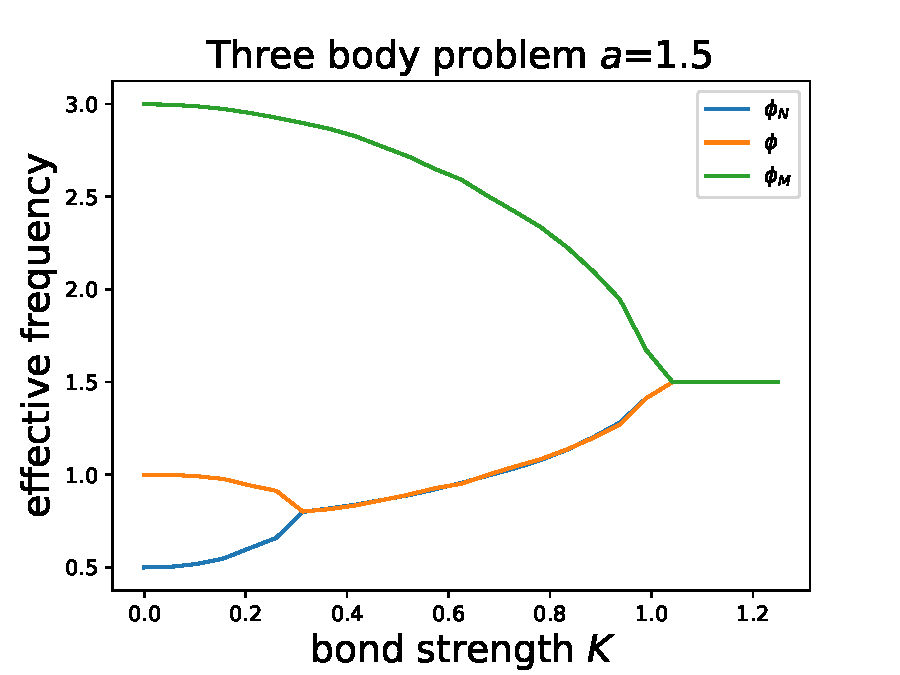
\includegraphics[keepaspectratio, scale=0.42]{images/three-body-prob-notapprox-a150.pdf}
        \subcaption[c]{$a=1.5,\ \Omega=-2,\ \omega=0.5$.\\3種類の同期状態を経ている.}
        \label{fig:3body-notapprox150}
    \end{minipage}
    \begin{minipage}[b]{0.47\linewidth}
      \centering
      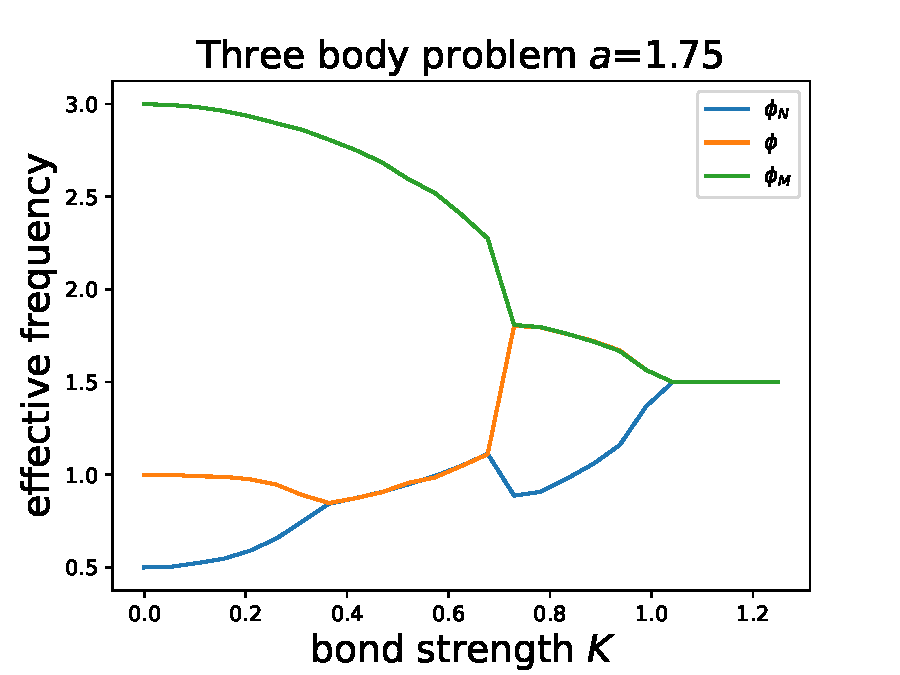
\includegraphics[keepaspectratio, scale=0.42]{images/three-body-prob-notapprox-a175.pdf}
      \subcaption{$a=1.75,\ \Omega=-2,\ \omega=0.5$.\\5種類の同期状態を経ている.}
      \label{fig:3body-notapprox175}
    \end{minipage}\\
    \begin{minipage}[b]{0.47\linewidth}
        \centering
        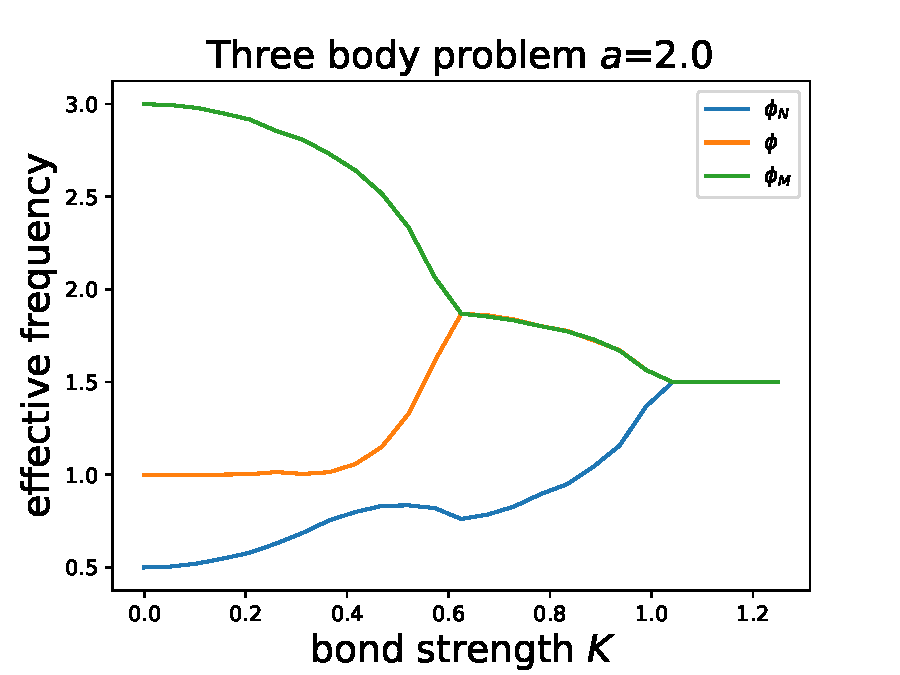
\includegraphics[keepaspectratio, scale=0.42]{images/three-body-prob-notapprox-a200.pdf}
        \subcaption{$a=2.0,\ \Omega=-2,\ \omega=0.5$.\\3種類の同期状態を経ている.}
      \label{fig:3body-notapprox200}
    \end{minipage}
    \begin{minipage}[b]{0.47\linewidth}
        \centering
        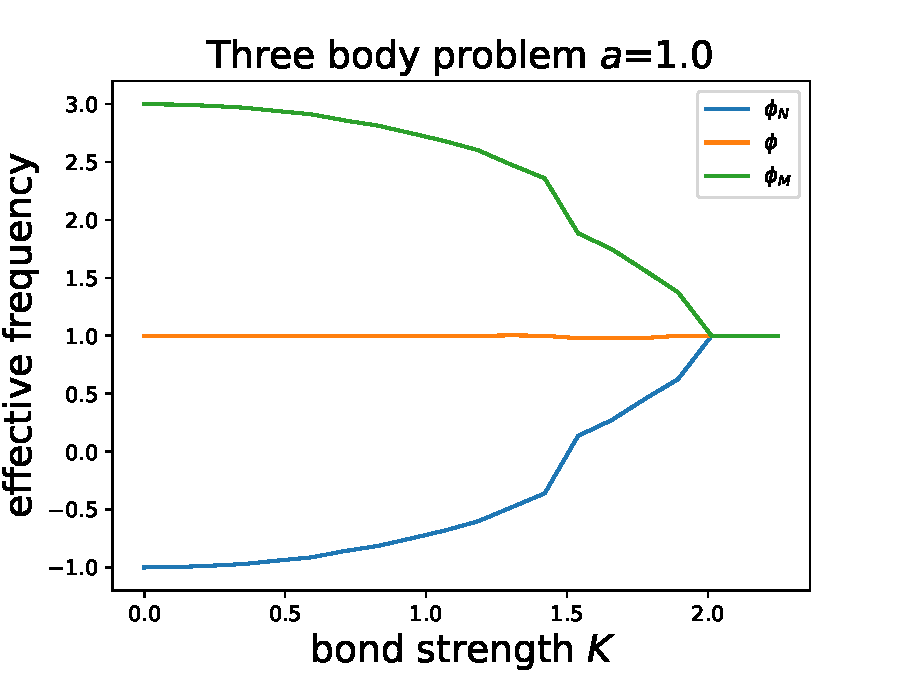
\includegraphics[keepaspectratio, scale=0.42]{images/three-body-prob-symmetry-a100.pdf}
        \subcaption{$a=1.0,\ \Omega=-2,\ \omega=2$.\\2種類の同期状態を経ている.}
        \label{fig:3body-symmetry}
    \end{minipage}
    \caption{様々なパラメータ$a,\ \Omega,\ \omega$で結合強度$K$を変化させたときの同期状態の変化}
    \label{fig:3body-abs}
\end{figure}
\clearcaptionsetup{figure}

最大で5つの同期状態が存在し,4つの臨界結合強度が存在することがわかった.
どのパターンの臨界結合強度も,図\ref{fig:3body-notapprox175}のパターンにおける臨界結合強度の一部が存在する場合として考えることができる.
つまり,図\ref{fig:3body-notapprox150}は$K=0.7$付近の臨界結合強度が2つとも存在せず$K=0.3,\ K=1.0$付近の臨界結合強度が存在する場合として解釈できる.
図\ref{fig:3body-notapprox175}は$K=0.7$付近の臨界結合強度が1つだけ存在し$K=1.0$付近の臨界結合強度が存在する場合として解釈できる.
そして,図\ref{fig:3body-symmetry}は一番大きい臨界結合強度だけが存在する場合として解釈できる.
よって,3体系のふるまいを理解する上では,図\ref{fig:3body-notapprox175}の場合の同期状態の変化及び臨界結合強度を解析するだけで十分である.

特に,次節以降の解析の都合,図\ref{fig:3body-notapprox175}と同様に最も多様に同期状態が変化するパラメータであり,
$|\Omega|\gg|\omega|$となる$a=4.0,\ \Omega=-2,\ \omega=0.05$の場合について注目する.
そのときの結合強度と実効振動数の関係を図\ref{fig:3body-state}に示す.

\begin{figure}[tbp]
\centering
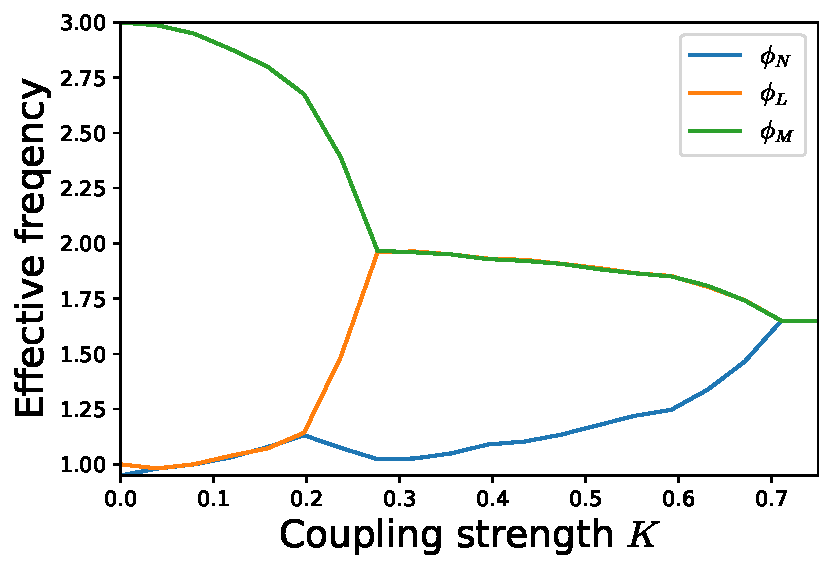
\includegraphics[width=105mm]{./images/three-body-prob.pdf}
\centering
\caption{3体ネットワークで$a=4.0,\ \Omega=-2,\ \omega=0.05$のしたときの結合強度$K$と実効振動数の関係.
$0\leq K\lesssim 0.05$では3体が非同期であり(phase 1),$0.03\lesssim K\lesssim 0.15$では固有振動数の近い2体が同期する($\phi_L=\phi_N$, phase 2).そして,$0.15 \lesssim K\lesssim 0.27$では鞍替えが起こり非同期になり(phase 3),$0.27\lesssim K\lesssim 0.7$では振動数の遠い2体が同期する($\phi_L=\phi_M$,\ phase 4).最後に$K\gtrsim 0.7$では3体が同期する(phase 5).}
\label{fig:3body-state}
\end{figure}

4つの臨界結合強度を分岐点として5つの同期状態に分岐することが分かる.
そこで,4つの臨界結合強度を小さい順にそれぞれ$K_1,\ K_2,\ K_3,\ K_4$とすると,次のようにまとめられる.
$0\leq K<K_1$では3体が非同期であり(phase 1),$K_1\leq K<K_2$では固有振動数の近い2体が同期する($\phi_L=\phi_N$,\ phase 2).そして,$K_2\leq K<K_3$では鞍替えが起こり非同期になり(phase 3),$K_3\leq K<K_4$では振動数の遠い2体が同期する($\phi_L=\phi_M$,\ phase 4).最後に$K\leq K_4$では3体が同期する(phase 5).

次節ではこれらの5つの同期状態が相平面上でどのように記述されるかを調べる.
\section{3体系の同期状態の相平面解析}
\label{sec:3body-phase-plane}
$x\coloneqq \phi_L-\phi_M,\ y\coloneqq\phi_L-\phi_N$というように位相差を取ると,式\eqref{eq:3body}から2本の位相差に関する方程式が得られる.
\begin{align}
    \label{eq:phase-diff}
    \begin{split}
    \dot{x}&=\Omega-K(2a\sin x+\sin y),\\
    \dot{y}&=\omega-K(a\sin x+2\sin y).
    \end{split}
\end{align}

図\ref{fig:3body-state}のそれぞれの同期状態に対応する$x$-$y$平面上の相図を図\ref{fig:phase}に示す.

\captionsetup[figure]{justification=centering}
\begin{figure}[tbp]
    \begin{minipage}[b]{0.47\linewidth}
      \centering
      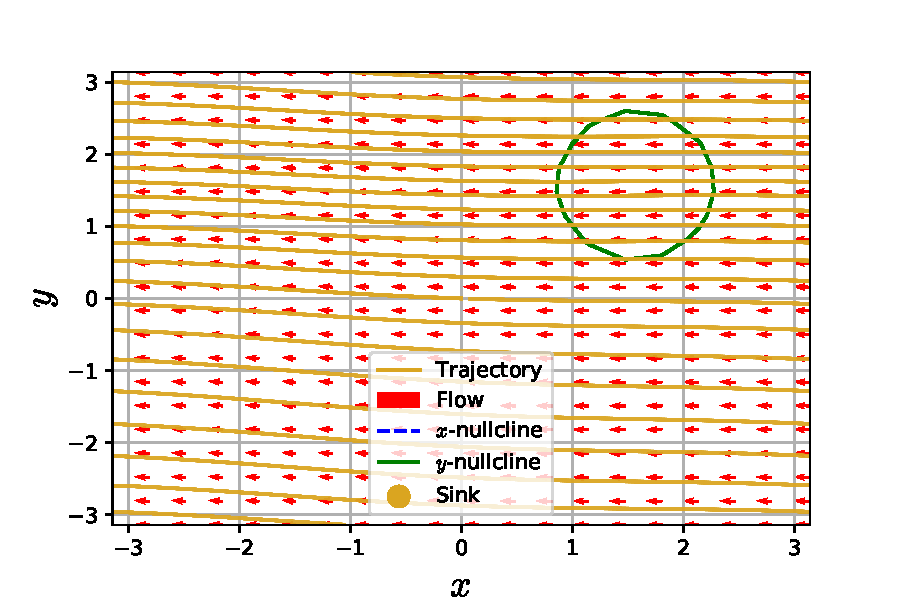
\includegraphics[keepaspectratio, scale=0.42]{images/phase_a4K2.pdf}
      \subcaption{$K=0.02$.3体が非同期.\\phase 1}
      \label{fig:phase-k2}
    \end{minipage}
    \begin{minipage}[b]{0.47\linewidth}
      \centering
      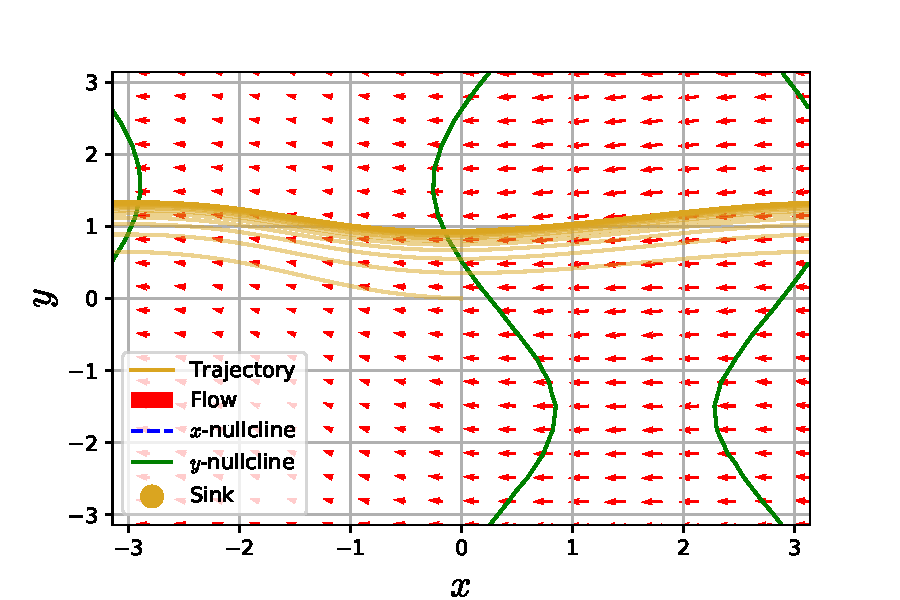
\includegraphics[keepaspectratio, scale=0.42]{images/phase_a4K10.pdf}
      \subcaption[c]{$K=0.1$.固有振動数が近いものと同期.\\phase 2}
      \label{fig:phase-k10}
    \end{minipage}\\
    \begin{minipage}[b]{0.47\linewidth}
      \centering
      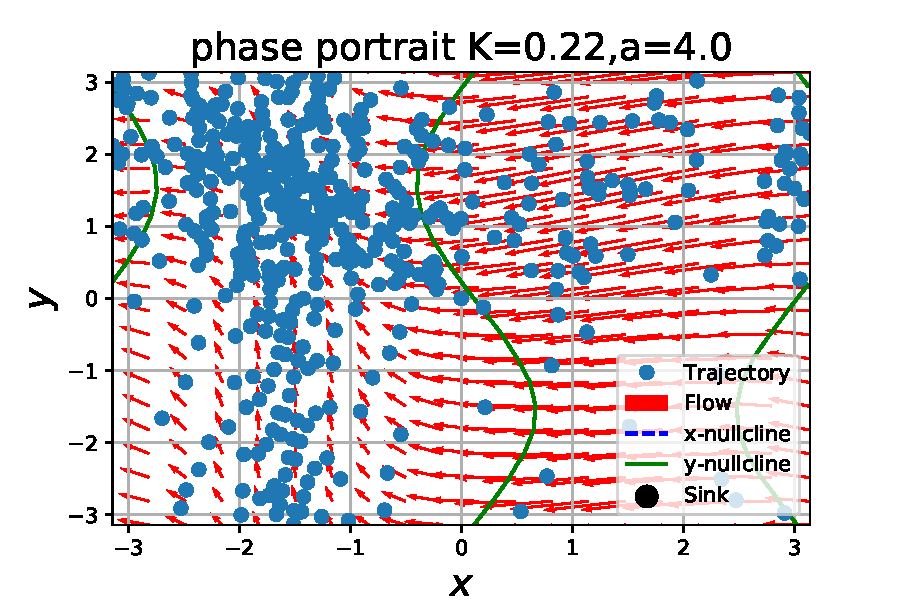
\includegraphics[keepaspectratio, scale=0.42]{images/phase_a4K22.pdf}
      \subcaption{$K=0.22$.同期が解除され3体が非同期.\\phase 3}
      \label{fig:phase-k22}
    \end{minipage}
    \begin{minipage}[b]{0.47\linewidth}
      \centering
      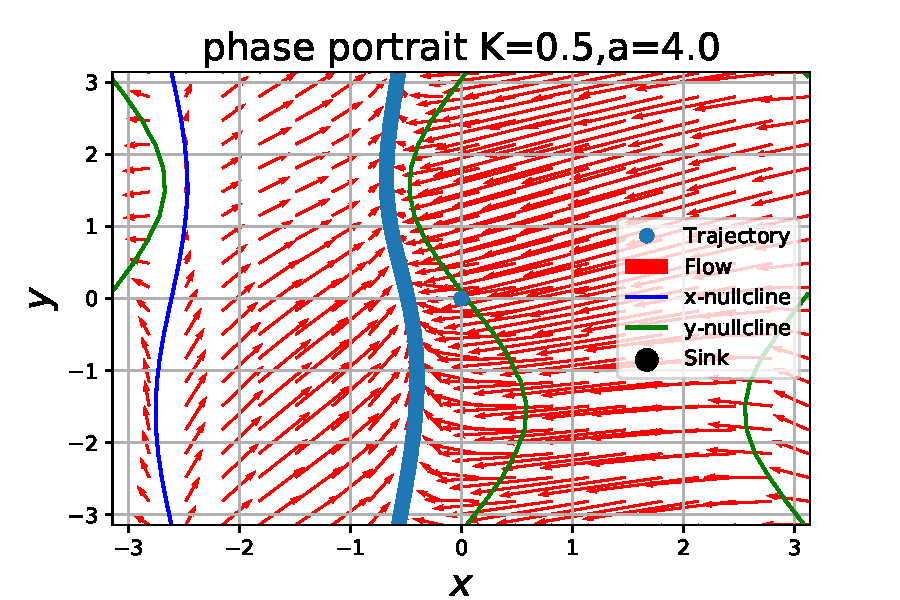
\includegraphics[keepaspectratio, scale=0.42]{images/phase_a4K50.pdf}
      \subcaption{$K=0.5$.固有振動数が遠いものと同期.\\phase 4}
      \label{fig:phase-k50}
    \end{minipage}\\
    \begin{minipage}[b]{0.47\linewidth}
      \centering
      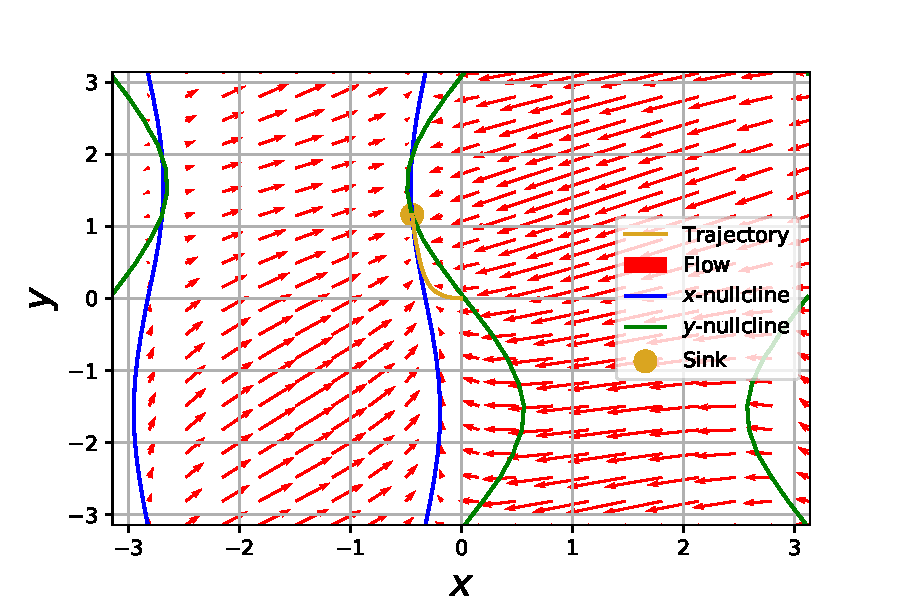
\includegraphics[keepaspectratio, scale=0.42]{images/phase_a4K80.pdf}
      \subcaption{$K=0.8$.3体とも同期.\\phase 5}
      \label{fig:phase-k80}
    \end{minipage}
    \caption{$a=4.0,\ \omega=0.1,\ \Omega=-2$における5つの同期状態における相図.\\
    ベクトル場,$x$-nullcline,$y$-nullcline,沈点,及び$(x,y)=(0,0)$から発する軌道を示している.}
    \label{fig:phase}
\end{figure}
\clearcaptionsetup{figure}

それぞれの同期状態は2本の位相差に関する方程式の安定解に対応し,それぞれ以下のような現象に対応する.
\begin{itemize}
    \item 
    2振動子の同期:任意の初期位相差から位相差$x,y$の片方のみが安定な$\mathbb{S}^1$と同相な周期軌道へ収束する.(図\ref{fig:phase-k10},\ \ref{fig:phase-k50})
    \item
    3振動子の同期:任意の初期位相差から位相差$x,y$の両方とも安定な平衡点へ収束する.(図\ref{fig:phase-k80})
    \item
    非同期:ほとんど確実に,安定な周期軌道が存在せず,$\mathbb{T}^2$全てを覆うような準周期軌道を描く.(図\ref{fig:phase-k2},\ \ref{fig:phase-k22})
\end{itemize}
以上の相平面解析の結果を元に,以降の節では4つの臨界結合強度を求める.
\section{臨界結合強度の近似解}
\label{sec:3body-critical}
    \subsection{固有振動数の近い2体との同期($K_1$,$K_2$)}
    \label{sec:3body-k12}
    本節では解析のために2つの振動数差が大きく異なるとし,以下の関係を仮定する.
    \begin{equation}
        \label{eq:assume}
        |\Omega|\gg|\omega|.
    \end{equation}
    固有振動数差$\Omega,\ \omega$に比べ,結合強度$K$が小さい状況($K\leq K_1$)では,以下の大小関係が成り立つ.
    \begin{equation}
        \label{eq:k1-approx}
        |\Omega|\gg|\omega|>K.
    \end{equation}
    また,
    結合強度$K$が固有振動数差$\Omega$に比べ小さく,固有振動数差$\omega$に比べ大きい状況($K\sim K_2$)では,以下の大小関係が成り立つ.
    \begin{equation}
        \label{eq:k2-approx}
        |\Omega|\gg K>|\omega|.
    \end{equation}
    式\eqref{eq:k1-approx},\ \eqref{eq:k2-approx}両方の状況とも,平均的に$x$は固有振動数$\Omega$で変化し,$y$は$\omega$($|\omega|\ll|\Omega|$)で変化する.
    よって,タイムスケールの分離が存在する.
    つまり,$\dot{x}=\Omega,\ y=z$($\dot{z}=\omega$)に対して,$K$に依存した周期外力を摂動として扱うような近似ができる.

    式\eqref{eq:phase-diff}において,無次元量$\tau\coloneqq\Omega t,\ \varepsilon\coloneqq\omega/\Omega,\ k=K/\Omega$を導入し,$S(x,y)=-a\sin x-2\sin y$とすると,位相差$y$の時間発展は以下のように表される.
    \begin{equation}
        \dv{y}{\tau}=\varepsilon+k S(x,y).
    \end{equation}

    このとき,$y$を以下のように近恒等変換する.
    \begin{equation}
        y=z+kh_1(z,\tau)+k^2h_2(z,\tau)+O(k^3).
        \label{eq:pertu-ytilde}
    \end{equation}
    ここで,$h_i$は$i=1,2,\ h_i(z+2\pi,\tau+2\pi)=h_i(z,\tau),\ h_i(z,0)=0$を満たす関数とする.

    一方,$x$については$k$の1次で展開すると以下のようになる.
    \begin{align}
        x&=\Omega t-\Omega k\int_0^t(2a\sin(x+\Omega s)+\sin (z+\omega s))\dd{s}+O(k^2)\notag\\ 
        &=\tau-\Omega k\left(\frac{2a}{\Omega}\sin\tau+\frac{\tau}{\Omega}\sin z+\frac{\omega \tau^2}{2\Omega^2}\cos z\right)+O(k^2,k\varepsilon^2).\label{eq:x-series}
    \end{align}
    最終行では,$\cos x(0)=0$となるように初期時刻$t=0$を定めたことに因る.
    
    式\eqref{eq:pertu-ytilde},\ \eqref{eq:x-series}を用いて,$S(x,y)$を$z,\ \tau$に関して展開する.
    \begin{align}
        S(x,y)&=-a\sin x-2\sin y\notag\\
        &=-a\sin\tau-2\sin z-2 kh_1\cos z\notag\\
        &+a\cos\tau\cdot \Omega k\left(\frac{2a}{\Omega}\sin\tau+\frac{\tau}{\Omega}\sin z+\frac{\omega \tau^2}{2\Omega^2}\cos z\right)+O(k^2,k\varepsilon^2)\notag\\
        &=-a\sin\tau-2\sin z\notag\\
        &+k\left(-2 \cos z\cdot h_1+a^2\sin 2\tau+a\tau\cos \tau\sin z+\frac{a\varepsilon \tau^2}{2}\cos \tau \cos z\right)+O(k^2,k\varepsilon^2).
    \end{align}
    さらに,$S_1\coloneqq-a\sin\tau-2\sin z,\ S_2\coloneqq a^2\sin 2\tau+a\tau\cos \tau\sin z+a\varepsilon \tau^2/2 \cdot\cos \tau \cos z$と定めると,
    \begin{equation}
        S(x,y)=S_1+k\pt_y S_1\cdot h_1+kS_2
    \end{equation}
    となる.
    式\eqref{eq:pertu-ytilde}を両辺$\tau$で微分すると,$\dot{\ast}=\dd{\ast}/\dd{\tau}$として,
    \begin{align}
        \dv{y}{\tau}&=\dot{z}+k(\dot{z}\partial_zh_1+\partial_\tau h_1)+k^2(\dot{z}\partial_zh_2+\partial_\tau h_2)+O(k^3)\notag\\
        &=(1+k\partial_zh_1+k^2\partial_zh_2)\dot{z}+k\pt_\tau h_1+k^2\pt_\tau h_2+O(k^3).
    \end{align}
    整理すると,以下のようになる.
    \begin{align}
        \dot{z}&=(1+k\pt_zh_1+k^2\pt_zh_2)^{-1}\left( \dv{y}{t}-k\pt_\tau h_1-k^2\pt_\tau h_2 \right)+O(k^3)\notag\\
        &=(1-k\pt_zh_1-k^2\pt_zh_2)\left(\varepsilon+kS_1+k^2 \pt_y S_1h_1+k^2S_2-k\pt_\tau h_1-k^2\pt_\tau h_2 \right)\notag\\
        &=\varepsilon+k(S_1-\pt_\tau h_1-\varepsilon\pt_zh_1)\!+\!k^2\left(\pt_y S_1h_1 -\pt_\tau h_2-\varepsilon\pt_zh_2 -\pt_zh_1(S_1-\pt_\tau h_1)+S_2\right).
    \end{align}
    $\dot{z}$が以下のように展開されるとする.
    \begin{equation}
        \dot{z}=\varepsilon+kH_1(z-\varepsilon \tau)+k^2H_2(z-\varepsilon \tau)+O(k^3).
    \end{equation}
    ここで,$z$が平均的に振動数$\omega$(無次元時間$\tau$では$\varepsilon$)で変動することから$H_1,\ H_2$が$z-\varepsilon \tau$に依存するものとした.
    
    このとき,$k$の1次を比較すると新たな変数$s$を用いて以下の式が成立する.
    \begin{equation}
        H_1(z-\varepsilon \tau)=S_1(z+\varepsilon s,\tau+s)-\pt_s h_1(z+\varepsilon s,\tau+s).
    \end{equation}
    $s=0$から$s=-\tau$で両辺積分すると,
    \begin{align}
        -\tau H_1(z-\varepsilon \tau)&=\int_0^{-\tau}\left(-a\sin(\tau+s)-2\sin(z+\varepsilon s)\right)\dd{s}+h_1(z,\tau)\notag \\
        &=a \sin\tau+\frac{2}{\varepsilon}(\cos (z-\varepsilon t)-\cos  z)+h_1(z,\tau)\notag\\
        &=a \sin\tau+\frac{2}{\varepsilon}(\cos z+\varepsilon \tau\sin z-\varepsilon^2\tau^2/2\cdot\sin z-\cos z)+h_1(z,\tau)+O(\varepsilon^2)\notag\\
        &=a \sin\tau+2\tau\sin z-\varepsilon \tau^2\cos z+h_1(z,\tau)+O(\varepsilon^2).
        \label{eq-h1-H1}
    \end{align}
    となり,$\tau=-2\pi$を代入すると,以下のようになる.
    \begin{align}
        2\pi H_1\left(z+ 2\pi\varepsilon\right)&=-4\pi\sin z-4\pi^2\varepsilon \cos z+O(\varepsilon^2)\notag\\
        H_1\left(z+2\pi\varepsilon\right)&=-2 \sin z-2\pi\varepsilon \cos z+O(\varepsilon^2).\label{eq:H1-approx}
    \end{align}
    また,式\eqref{eq:H1-approx}の左辺を$z$まわりに$\varepsilon$について展開すると,以下のようになる.
    \begin{equation}
        H_1\left(z+2\pi\varepsilon\right)=H_1(z)+H_1'(z) 2\pi\varepsilon+O(\varepsilon^2).
        \label{eq:H1-taylor}
    \end{equation}
    式\eqref{eq:H1-approx}と式\eqref{eq:H1-taylor}を$\varepsilon$について比較すると,
    \begin{equation}
        \label{eq:nit-H1}
        H_1(z)=-2\sin z+2\pi\varepsilon \cos z+O(\varepsilon^2)
    \end{equation}
    が得られる.
    式\eqref{eq-h1-H1}に代入すると,
    \begin{align}
        h_1(z,\tau)&=2\tau\sin(z-\varepsilon \tau)-2\pi\varepsilon \tau\cos(z-\varepsilon \tau)-a\sin\tau-2\tau\sin z+\varepsilon \tau^2\cos z\notag\\
        &=2\tau(\sin z-\varepsilon \tau\cos z-\sin z)-a\sin\tau+\varepsilon(-2\pi \tau+\tau^2)\cos z+O(\varepsilon^2)\notag\\
        &=-a\sin\tau-\varepsilon(2\pi \tau+\tau^2)\cos z+O(\varepsilon^2)
    \end{align}
    となる.

    次に$\dot{z}$の$k$の2次を比較し,$h_1$を代入する.
    \begin{align}
        \begin{split}
            H_2(z-\varepsilon \tau)=&\ \pt_y S_1h_1 -\pt_\tau h_2-\varepsilon\pt_zh_2 -\pt_zh_1(S_1-\pt_\tau h_1)+S_2\\
            =&-2\cos (z+\varepsilon s)\left( -a\sin(\tau+s)-\varepsilon(2\pi (\tau+s)+(\tau+s)^2) \cos (z+\varepsilon s) \right)\\
            % +&\  a^2\sin 2(\tau+s)+a(\tau+s)\cos (\tau+s)-\pt_\tau h_2+O(\varepsilon^2)\\
            +&\ a^2\sin 2(\tau+s)+a(\tau+s)\cos (\tau+s)\sin (z+\varepsilon s)\\
            +&\ \frac{a\varepsilon (\tau+s)^2}{2}\cos (\tau+s) \cos (z+\varepsilon s)-\pt_\tau h_2+O(\varepsilon^2)\\
            +&\ \varepsilon(2\pi(\tau+s)+(\tau+s)^2)\sin (z+\varepsilon s) \\
            &\left( -a\sin(\tau+s)-2\sin (z+\varepsilon s) +a\cos(\tau+s)\right.\\
            &\left.+\varepsilon(2\pi +2(\tau+s))\cos (z+\varepsilon s)\right).
        \end{split}
    \end{align}
    両辺$s=0$から$s=-\tau$で積分して,$\sin\tau\sim 0,\ \cos\tau\sim 1$とすると,
    \begin{align}
        -\tau H_2(z-\varepsilon \tau)&=2a\cdot -\varepsilon \tau\sin z+4\pi\varepsilon\left( -\frac{\tau^2}{4} -\frac{\tau^2}{4}\cos 2z\right)+2\varepsilon\left( -\frac{\tau^3}{6} -\frac{\tau^3}{6}\cos 2 z\right)\notag\\
        &-2\pi a\varepsilon\cdot\left(\tau\sin z\right)+2\pi a\varepsilon\left(-\varepsilon \tau\cos z\right)\notag\\
        &-4\pi\varepsilon\left(-\frac{\tau^2}{4}+\frac{\tau^2}{4}\cos 2 z\right)-2\varepsilon\left( -\frac{\tau^3}{6} +\frac{\tau^3}{6}\cos 2z\right)+O(\varepsilon^2)\notag\\
        &-a\varepsilon\left( \tau^2\sin z \right)+a\varepsilon\left( -2\tau^2\sin z \right)\notag\\
        &+\frac{a^2}{2}\left( \cos 2\tau-1\right)+a\tau(a+\cos z)\notag\\
        &+\frac{a\varepsilon}{2}(-\tau\sin\tau+1-\cos\tau)\cos z\notag\\
        &=-2a\varepsilon \tau\sin z-2\pi\varepsilon\tau^2\cos 2 z-\frac{2}{3}\varepsilon\tau^3\cos 2z\notag\\
        &-2\pi a\varepsilon \tau\sin z-3a\varepsilon\tau^2\sin z+a\tau(a+\cos z)+O(\varepsilon^2)
    \end{align}
    となる.$\tau=-2\pi$を代入して整理すると以下のようになる.
    \begin{align}
        \begin{split}
            &H_2(z+2\pi\varepsilon )=-a(a+\cos z)+O(\varepsilon^2)\\
            &+2\varepsilon\left( a\sin z-2\pi^2\cos2 z+\frac{4\pi^2}{3} \cos 2 z+\pi a\sin z-3\pi a\sin z\right).
        \end{split}
    \end{align}
    $H_1$と同様に$z$まわりに$\varepsilon$に関して展開し,$\varepsilon$について比較すると,以下の式が得られる.
    \begin{equation}
        \label{eq:nit-H2}
        H_2(z)=-a(a+\cos z)+2\varepsilon\left( (1-3\pi)a\sin z-\frac{2\pi^2}{3} \cos 2 z\right)+O(\varepsilon^2).
    \end{equation}

    以上で,位相差$y$の近恒等変換$z$の従う微分方程式を近似的に求めることができる.
    よって,$z$が安定解を持つ条件を求めることで$y$が安定解を持つ条件を求めることができる.
    
    まず,式\eqref{eq:k1-approx}の状況では,
    \begin{equation}
        \dot{z}=\varepsilon-2k\sin z
        \label{eq:z-k1-approx}
    \end{equation}
    となる.これは,式\eqref{eq:phase-diff}に対し$x$の周期で平均化を行った(つまり,$\sin x\sim 0$)式である.
    式\eqref{eq:z-k1-approx}で$z$が安定解を持つ条件は,
    \begin{equation}
        k\geq\frac{\varepsilon}{2}
    \end{equation}
    となり,臨界結合強度$K_1$は,
    \begin{equation}
        \label{eq:K1-approx}
        K_1=\frac{\omega}{2}
    \end{equation}
    となる.

    次に,式\eqref{eq:k2-approx}の状況を考える.
    閉形式で$K_2$を求めるため$|a\varepsilon k^2| \ll 1,\ |\varepsilon k|\ll 1$を仮定すると,$k$の2次まで考えると$z$は以下のような微分方程式に従う.
    \begin{align}
        \label{eq:z-k2-approx}
        \begin{split}
            \dot{z}&=\varepsilon-2k\sin z-k^2a(a+\cos  z)\\
            &=\varepsilon-a^2k^2-k\sqrt{4+a^2k^2}\sin ( z-\alpha)\quad(\alpha:\mathrm{const}).
        \end{split}
    \end{align}
    $z$が安定解を持つ条件は,
    \begin{align}
        |\varepsilon-a^2k^2|&\leq k\sqrt{4+a^2k^2}\notag\\
        0\leq |k|&\leq \sqrt{\frac{1}{a^4-a^2}\left(2+a^2\varepsilon+\sqrt{(2+a^2\varepsilon)^2-\varepsilon^2(a^4-a^2)}\right)}
    \end{align}
    となり,臨界結合強度$K_2$は,
    \begin{equation}
        \label{eq:K2-approx}
        K_2=|\Omega|\cdot\sqrt{\frac{1}{a^4-a^2}\left(2+a^2\varepsilon+\sqrt{(2+a^2\varepsilon)^2-\varepsilon^2(a^4-a^2)}\right)}
    \end{equation}
    となる.
    ただし,$K_2$が実数となるためには$\varepsilon$及び$a$が以下の条件を満たす必要がある.
    \begin{equation}
        a^2\varepsilon^2+4a^2\varepsilon+4\geq 0
    \end{equation}
    \subsection{固有振動数の遠い2体との同期($K_3$)}
    \label{sec:3body-k3}
    固有振動数の遠い2体との同期については,以下の命題\ref{prop:suff}により,
    \begin{equation}
        \label{eq;:K2-approx}
        K_3\lessapprox \frac{|\Omega|}{2a-1}\coloneqq K'_3
    \end{equation}
    を得た.
    \begin{proposition}
        \label{prop:suff}
        トーラス$\mathbb{T}^2$上の自律系
        \begin{align}
            \label{eq:prop-2phase}
            \begin{split}
                \dot{x}&=\Omega-K(2a\sin x+\sin y),\\
                \dot{y}&=\omega-K(a\sin x+2\sin y)
            \end{split}
        \end{align}
        において,平衡点を持たず,任意の$y$に対し$\dot{x}=0$が解を持つならば,
        つまり,$K,a$が
        \begin{equation*}
            K\geq \frac{|\Omega|}{2a-1}
        \end{equation*}
        を満たすならば,
        2つの安定,不安定な$x$-$\mathrm{nullcline}$付近に$\mathbb{S}^1$と同相な安定,不安定な周期解がそれぞれ1つずつ存在し,任意の点から発する軌道は2つの周期解のどちらかに収束する.
    \end{proposition}
    まず,以下の補題を示す.
    \begin{lemma}
        \label{lemma:annulus}
        命題\ref{prop:suff}の状況で
        安定な$x$-nullclineの$x$座標の最大値・最小値をそれぞれ$x_{\max},\ x_{\min}$とし,$D=[x_{\min},x_{\max}]\times (-\pi,\pi ]\subset\mathbb{T}^2$とする.
        このとき,円筒領域$D$内に$\mathbb{S}^1$に同相な安定な周期解がただ一つ存在する.        
    \end{lemma}
    \begin{proof}
        まず,$D$内の任意の点から発する軌道は$D$内に留まる.
        なぜなら,$D$内の点から発して$D$外に出る軌道が存在すると仮定すると$D$の境界上で$D$外の流れを持つが,図\ref{fig:phase-k50}よりそのような点は存在しないからである.

        そして,命題\ref{prop:suff}の仮定より平衡点は存在せず,$D$は円環に同相でトーラス$\mathbb{T}^2$と同相でない.\\
        以上より,Poincar\'{e}-Bendixsonの定理の一般化(定理\ref{thm:poiben-gen})から$D$内に$\mathbb{S}^1$に同相な周期解が存在する.
        
        また,その周期解は$y$方向の流れが一定であることから,安定な$x$-nullclineと交差し,安定な周期解となる.
        特に,安定な周期解は$x$-nullclineが$x_{\max}$から$x_{\min}$に変化する間とその逆で1回ずつ交わる.
        このことと$x$-nullclineを挟んで流れが変化することから安定な周期解はただ一つ存在する.    
    \end{proof}
    次に命題\ref{prop:suff}の証明を示す.
    \begin{proof}
        補題\ref{lemma:annulus}と式\eqref{eq:prop-2phase}の座標・時刻に対する対称性から,安定な$x$-nullclineと不安定な$x$-nullclineの付近にそれぞれ安定,不安定な周期解$\gamma_a,\ \gamma_b$を持つ.

        他に周期解$\gamma$が存在すると仮定すると,$\gamma$は$\gamma_a,\ \gamma_b$と交わることはないので,任意の$y\in(-\pi,\pi]$に対し,ある$x\in(-\pi,\pi]$が存在して,$(x,y)\in\gamma$となる.
        また,そのような周期解は$x$-nullclineと交わる必要がある.なぜなら,$x$-nullclineと交わるまで流れの$x$成分の符号が変わらないので必ず$x$-nullclineに到達するからである.
        しかし,補題\ref{lemma:annulus}より,1つの$x$-nullclineは1つの周期解としか交わらないため矛盾する.

        最後に,Poincar\'{e}-Bendixsonの定理の一般化(定理\ref{thm:poiben-gen})により,任意の点から発する軌道は$\gamma_a,\ \gamma_b$のいずれかに収束する.
    \end{proof}

    \subsection{3体の同期($K_4$)}
    \label{sec:3body-k4}
    本節では$2\Omega\leq\omega,\ 2\omega\geq\Omega$を仮定するが,それ以外の場合も同様の議論が成り立つ.

    式\eqref{eq:phase-diff}が(双曲的)平衡点を持つとき,
    \begin{alignat*}{2}
        x_1&=\arcsin \frac{2\Omega-\omega}{3aK}<0,&\quad x_2&=-\pi-\arcsin \frac{2\Omega-\omega}{3aK},\\
        y_1&=\arcsin \frac{2\omega-\Omega}{3K}>0,&\quad y_2&=\pi-\arcsin \frac{2\omega-\Omega}{3K}
    \end{alignat*}
    とすると,平衡点は,
    \begin{equation*}
        (x,y)=(x_1,y_1),\ (x_1,y_2),\ (x_2,y_1),\ (x_2,y_2).
    \end{equation*}
    となる.
    よって,平衡点の存在条件は,
    \begin{equation}
        K\geq \frac{|2\Omega-\omega|}{3a}\ \cap \ K\geq \frac{|\Omega-2\omega|}{3}
    \end{equation}
    となる.
    また,式\eqref{eq:phase-diff}のヤコビ行列$J$は
    \begin{align*}
        J=-K\begin{pmatrix}
            2a\cos x&\cos y\\
            a\cos x&2\cos y
        \end{pmatrix}
    \end{align*}
    であり,
    \begin{align}
        \tr J&=-K(2a\cos x+2\cos y),\\
        \det J&=3aK^2\cos x\cos y,\\
        (\tr J)^2-4\det J&=K^2(2a\cos x-2\cos y)^2> 0
    \end{align}
    である.
    ここで,$\cos x_1>0,\ \cos x_2<0,\ \cos y_1>0,\ \cos y_2<0$及び$a>0,\ K>0$より,
    \begin{alignat*}{2}
        \left.\det J \right|_{(x,y)=(x_1,y_1)}&>0, &\quad  \left.\tr J \right|_{(x,y)=(x_1,y_1)}&<0,\\
        \left.\det J \right|_{(x,y)=(x_1,y_2)}&<0, & &\\
        \left.\det J \right|_{(x,y)=(x_2,y_1)}&<0, & &\\
        \left.\det J \right|_{(x,y)=(x_2,y_2)}&>0, &\quad  \left.\tr J \right|_{(x,y)=(x_2,y_2)}&>0
    \end{alignat*}
    となるため,線形安定性から$(x_1,y_1)$は沈点,$(x_1,y_2),\ (x_2,y_1)$は鞍点,$(x_2,y_2)$は源点となる.
    実際,図\ref{fig:phase-k80}では平衡点は源点,2つの鞍点,沈点に分かれている.
    このとき,源点から2つの鞍点へ,2つの鞍点から沈点への流れがあるので,鞍点の安定多様体と交わるような Limit Cycle は存在しない.
    また,全ての平衡点は$x$-nullcline,\ $y$-nullclineの交点であるので,源点を囲うような Limit Cycle も存在しない.

    これまでの議論は双曲的平衡点が4つ存在する場合について述べたものであるが,非双曲的平衡点が2つ,つまり$x_1=x_2$もしくは$y_1=y_2$のときも,ベクトル場はほとんど変わらないことから同様の議論が成り立つ.

    よって,平衡点を持つとき,周期解は持たず,Poincar\'{e}-Bendixson の定理の一般化(定理\ref{thm:poiben-gen})から任意の点から発する軌道は平衡点へ収束する.
    特に,平面上のほとんど全ての点から発する軌道は沈点に収束する.

    以上より,3体が同期する臨界結合強度$K_4$は,
    \begin{equation}
        \label{eq:K4-approx}
        K_4=\max\left(\frac{|2\Omega-\omega|}{3a},\frac{|\Omega-2\omega|}{3}\right)
    \end{equation}
    となる.
    
    \subsection{臨界結合強度のまとめ}
    \label{sec:3body-summary}
    \ref{sec:3body-k12},\ \ref{sec:3body-k3},\ \ref{sec:3body-k4}節で示したように,臨界結合強度$K$は結合強度比$a$の関数として求められる.
    \begin{align}
        \label{eq:3body-matome}
        \begin{split}
            K_1&=\frac{\omega}{2},\\
            K_2&=|\Omega|\cdot\sqrt{\frac{1}{a^4-a^2}\left(2+a^2\varepsilon+\sqrt{(2+a^2\varepsilon)^2-\varepsilon^2(a^4-a^2)}\right)},\\
            K'_3&=\frac{|\Omega|}{2a-1},\\
            K_{41}&=\frac{|2\Omega-\omega|}{3a},\\
            K_{42}&=\frac{|\Omega-2\omega|}{3},\\
            K_4&=\max\left(K_{41},K_{42}\right).
        \end{split}
    \end{align}

    臨界結合強度から次のような定性的な同期現象の理解が得られる.
    固有振動数が近く枝が多いほど同期しやすい.
    そして,2つの集団との間の枝の本数の比がある程度偏っていて,結合強度がある程度強いとき,3体全体の同期や鞍替えが起こる.
    
    また,$K'_3\geq K_4$から固有振動数の離れた振動子との同期が起こる,つまり,鞍替え現象が発生するための結合強度比$a$の十分条件も求まる.
    \begin{equation}
        \label{eq:a-ast1}
        a\geq \frac{|2\Omega-\omega|}{|4\Omega-2\omega|-3|\Omega|}= 2-3|\varepsilon|+O(|\varepsilon|^2)\coloneqq a^\ast_1.    
    \end{equation}
    このとき,$a=a^\ast_1$で$K'_{3}(a^\ast_1)=K_{41}(a^\ast_1)=K_{42}(a^\ast_1)$となる.
    $a^\ast_1$を境に図\ref{fig:3body-notapprox150}の同期状態変化パターンから図\ref{fig:3body-notapprox175}に変化する.

    さらに,$K_1\geq K'_3$から固有振動数の近い振動子との同期が起こらずに固有振動数の離れた振動子との同期が起こる,つまり,鞍替え現象が発生しなくなるための結合強度比$a$の必要条件も求まる.
    \begin{equation}
        \label{eq:a-ast2}
        a\geq \frac{2|\Omega|+|\omega|}{2|\omega|}\coloneqq a^\ast_2.    
    \end{equation}
    $a^\ast_2$を境に図\ref{fig:3body-notapprox175}の同期状態変化パターンから図\ref{fig:3body-notapprox200}に変化する.

    式\eqref{eq:3body-matome}の正当性を確かめるため,$K$-$a$平面における同期状態の分岐図を描くことを考える.
    そして,各状態の境界が臨界結合強度$K_1,\ K_2,\ K_3,\ K_4$で記述される曲線となっていることを確認する.

    $K$-$a$平面における同期状態の分岐図を図\ref{fig:3body-phase}に示す.
    求めた臨界結合強度の近似解が境界をうまく近似できていることがわかる.
    また,$a^\ast_1\simeq 2$を境に結合強度に対する同期状態変化パターンが変化していることもわかる.
    加えて,$|\Omega|\gg|\omega|$の場合は図\ref{fig:3body-notapprox150},\ \ref{fig:3body-notapprox175},\ \ref{fig:3body-notapprox200}の同期状態変化パターンしか存在しないこともわかる.
    $K_2$で$K$が大きい場合に境界から離れているのは,$K_2$を求めるために利用した$k=K/\Omega$が小さいという近似が成り立たなくなるためであると思われる.

    \begin{figure}[tbp]
    \centering
    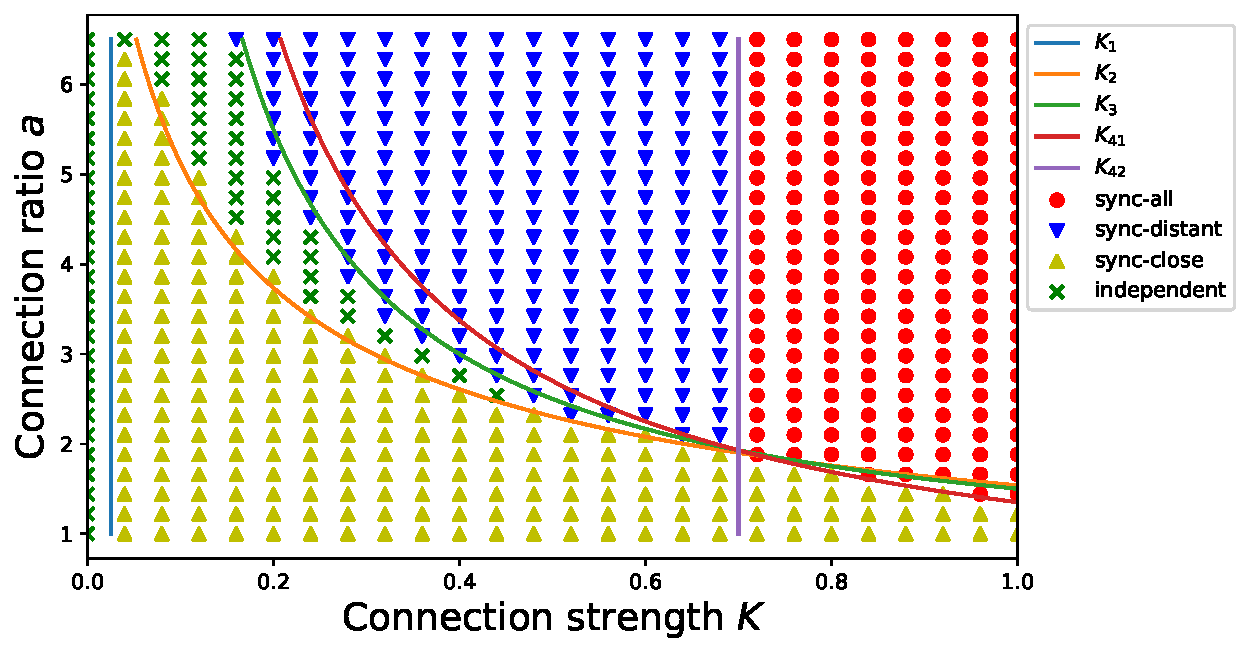
\includegraphics[width=135mm]{images/three-body-phase.pdf}
    \centering
    \caption{$\Omega=-2,\ \omega=0.05$のときの結合強度$K$,結合強度$a$における3体系の同期状態を表す分岐図.
    各格子点に対し,3体全体の同期・固有振動数の離れた振動子との同期・固有振動数の近い振動子との同期・3体とも非同期の4状態を示している.
    また,\ref{sec:3body-k12},\ \ref{sec:3body-k3},\ \ref{sec:3body-k4}節で求めた臨界結合強度の近似をそれぞれ重ねて示している.
    }
    \label{fig:3body-phase}
    \end{figure}

\subsection{一般の集団サイズをもつ3体系}
\label{sec:3body-general}
これまでの節では,鞍替えに関わる3つ集団のサイズ$L,\ M,\ N$について,$L=1,\ M=1,\ N=1$を仮定した式\eqref{eq:3body}について解析を行ってきた.
しかし,一般のネットワークにおける枝の増加・減少に伴う同期状態の変化を説明する上では,$L=1,\ M=1,\ N=1$の理論では不十分である.
そこで,本節では一般の$L,\ M,\ N$について同様の議論を行う.

まず,式\eqref{eq:3body-default}について,$a=m/n$として,$\tilde{K}=n\lambda/L$,$\tilde{M}=M/L$,$\tilde{N}=N/L$というように結合強度及び集団のサイズを定義し直すと以下のようになる.
\begin{align}
    \label{eq:3body-general}
    \begin{split}
        \dot{\phi}_L&=\omega_L+\tilde{K}\sin\left( \phi_N-\phi_L \right)+a\tilde{K}\sin\left( \phi_M-\phi_L \right),\\
        \dot{\phi}_M&=\omega_M+\frac{a\tilde{K}}{\tilde{M}}\sin\left( \phi_L-\phi_M \right), \\
        \dot{\phi}_N&=\omega_N+\frac{\tilde{K}}{\tilde{N}}\sin\left( \phi_L-\phi_N \right).    
    \end{split}
\end{align}

式\eqref{eq:3body-general}においても,\ref{sec:3body-synchro-state}節と同様にパラメータ$a,\ \tilde{K},\ \tilde{M},\ \tilde{N}$を変化させることで同期状態が変化することが期待される.
3体系について,様々な振動数差$\Omega\coloneqq\omega_L-\omega_M,\ \omega\coloneqq\omega_L-\omega_N$に対し,パラメータ$a,\ L,\ M,\ N$を様々な値で固定し,結合強度$\tilde{K}$を変化させたときの同期状態の変化を調べた.
すると,\ref{sec:3body-synchro-state}節と同様に,図\ref{fig:3body-abs}で見られた4つの同期状態の変化パターンを示すことがわかった.

続いて,\ref{sec:3body-phase-plane}節と同様に,3体系の同期状態と2つの位相差の相平面上の安定解との対応を調べる.
式\eqref{eq:phase-diff}と同様に,$x=\phi_L-\phi_M,\ y=\phi_L-\phi_N$という位相差を定義すると,式\eqref{eq:3body-general}から以下の$x,\ y$に関する2本の微分方程式が得られる.
\begin{align}
    \label{eq:phase-diff-general}
    \begin{split}
        \dot{x}&=\Omega-\tilde{K}\left( a\left(1+\frac{1}{\tilde{M}}\right)\sin x +\sin y\right),\\
        \dot{y}&=\omega-\tilde{K}\left( a\sin x +\left(1+\frac{1}{\tilde{N}}\right)\sin y\right).
    \end{split}
\end{align}

図\ref{fig:3body-state}で見られた3つの同期状態は,\ref{sec:3body-phase-plane}節と同様に式\eqref{eq:phase-diff-general}における安定解に対応する.
また,$x$-$y$平面における相図は図\ref{fig:phase}と同様の幾何学的性質を示す.
よって,\ref{sec:3body-critical}節と同様の手法で4つの臨界結合強度を求めることができ,以下が得られる.
\begin{align}
    \label{eq:3body-matome-general}
    \begin{split}
        K_1&=\frac{|\omega|}{1+1/\tilde{N}},\\
        K_2&=|\Omega|\cdot\sqrt{\frac{1}{a^4-a^2}\left((1+1/\tilde{N})^2/2+a^2\varepsilon+\sqrt{((1+1/\tilde{N})^2/2+a^2\varepsilon)^2-\varepsilon^2(a^4-a^2)}\right)},\\
        K'_3&=\frac{|\Omega|}{a(1+1/\tilde{M})-1}\gtrapprox K_3,\\
        K_4&=\max\left\{\frac{|(1+1/\tilde{N})\Omega-\omega|}{a(1/\tilde{N}+1/\tilde{M}+1/\tilde{N}\tilde{M})},\frac{|\Omega-(1+1/\tilde{M})\omega|}{(1/\tilde{N}+1/\tilde{M}+1/\tilde{N}\tilde{M})}\right\}.
    \end{split}
\end{align}
ただし,$K_1,\ K_2$については,$\Omega\gg\omega$を仮定し求めた.また,式\eqref{eq:3body-matome-general}で$\tilde{N}=1,\ \tilde{M}=1$としたものは式\eqref{eq:3body-matome}に一致することに注意せよ.

集団サイズ$N,\ M$を考慮した臨界結合強度についても同期現象の定性的な理解が得られる.
実効振動数が近い集団$\Omega_N$のサイズが小さく,実効振動数の差$|\omega|$が小さいほど,実効振動数の近い集団と同期しやすい.
実効振動数が近い集団$\Omega_N$と同期していた振動子集団$\Omega$は,$\Omega_N$のサイズ$N$が大きく,実効振動数が離れた集団$\Omega_M$との間に枝が多く,$\Omega_M$との振動数差$|\Omega|$が小さいほど,$\Omega_M$に引き寄せられ,同期が解除されやすい.
ここで,吸引する振動数集団$\Omega_M$のサイズ$M$には依らないことに注意.
また,実効振動数が離れた集団$\Omega_M$のサイズ$M$が小さく,$\Omega_N$に比べて枝が多く繋がっており,実効振動数の差$\Omega$が小さいほど,$\Omega_M$と同期しやすく,$\Omega_N$から$\Omega_M$に鞍替えしやすい.
そして,振動子集団$\Omega_N$のサイズ$N$がある程度小さく,結合強度比$a$がある程度大きいと3体全体が同期しやすい.

\section{3体系の適用例}
本節では3体系による同期状態の解析の例を示す.

まず,図\ref{fig:cutting_N6K1}において鞍替えの起こる$m=5$のときを用いる.
そのときのネットワーク及び3体系を適用する場合の集団の分割を図\ref{fig:cutting_N6-m5}に示す.
node 0, 1, 2 は固有振動数$-1$であり,node 3, 4, 5 は固有振動数$-1$である.全体が同期した$m=4$から赤で示した node 1 と node 2 をつなぐ枝が追加されることで$m=5$となる.\\
このとき,$\Omega_M=\{0,4,5\},\ \Omega_L=\{1\},\ \Omega_N=\{2\}$として振動子を分割すると3体系として計算することができる.
実際,$K=1$のとき,集団間の枝を無視すると各集団内の振動子は同期する.
$\Omega_M$は実効振動数$\omega_M=1/3$,サイズ$M=3$の集団で,$\Omega_L$は実効振動数$\omega_M=-1$,サイズ$L=1$の集団で,$\Omega_N$は実効振動数$\omega_N=-1$,サイズ$N=1$の集団である.

この集団では$|\Omega|=4/3\gg|\omega|=0$より臨界結合強度を求めることができる.
式\eqref{eq:phase-diff-general}におけるパラメータは$a=1,\ \tilde{M}=3,\ \tilde{N}=1$であるから,
$K_1=0,\ K_4=4/3$であり,$K_2>K_4,\ K_3>K_4$となり$K_2,\ K_3$は定義されない.
よって,式\eqref{eq:phase-diff-general}で結合強度をスケーリングしたことに注意して,図\ref{fig:cutting_N6K1}の結合強度$K=L\tilde{K}/n$が
\begin{equation*}
    0\leq \tilde{K}<\frac{4}{3}
\end{equation*}
を満たすとき,$\Omega_L$及び$\Omega_N$のみが同期し,
\begin{equation*}
    \tilde{K}\geq \frac{4}{3}
\end{equation*}
のとき,3つの集団全体が同期する.

図\ref{fig:cutting_N6K1}では$K=\tilde{K}=1$なので,元々同期していた$\Omega_M$ではなく,実効振動数の近い$\Omega_N$と同期する.つまり,$\Omega_M$から$\Omega_N$への鞍替えが起こる.また,結合強度を$K\geq 4/3$にすると全体が同期することも分かる.

\begin{figure}[tbp]
\centering
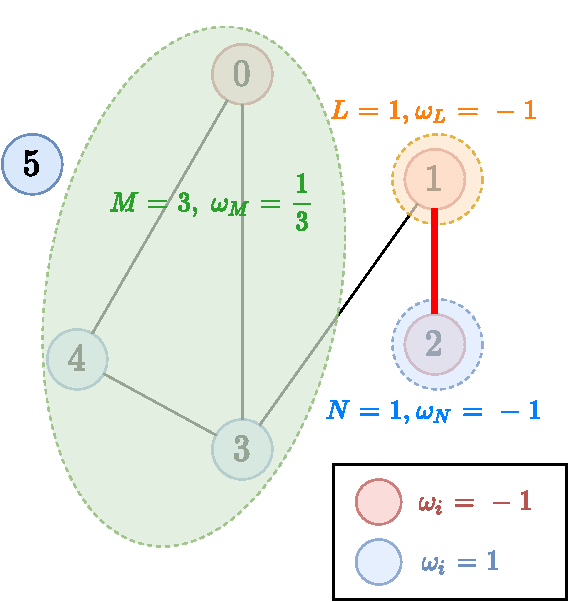
\includegraphics[width=70mm]{images/cutting_N6_drawio.pdf}
\centering
\caption{図\ref{fig:cutting_N6K1}における$m=5$のときのネットワーク.
node 0, 1, 2 は固有振動数$-1$であり,node 3, 4, 5 は固有振動数$-1$である.全体が同期した$m=4$から赤で示した node 1 と node 2 をつなぐ枝が追加されることで$m=5$となる.\\
このとき,$\Omega_M=\{0,4,5\},\ \Omega_L=\{1\},\ \Omega_N=\{2\}$として振動子を分割すると3体系として計算することができる.実際,$K=1$のとき,集団間の枝を無視すると各集団内の振動子は同期する.
$\Omega_M$は実効振動数$\omega_M=1/3$,サイズ$M=3$の集団で,$\Omega_L$は実効振動数$\omega_M=-1$,サイズ$L=1$の集団で,$\Omega_N$は実効振動数$\omega_N=-1$,サイズ$N=1$の集団である.}
\label{fig:cutting_N6-m5}
\end{figure}

次に,図\ref{fig:cutting_N6K1}と同じ$n=6$のネットワークであって3体系を有効に活用できる例を図\ref{fig:3body-application}に示す.

\begin{figure}[tbp]
    \centering
    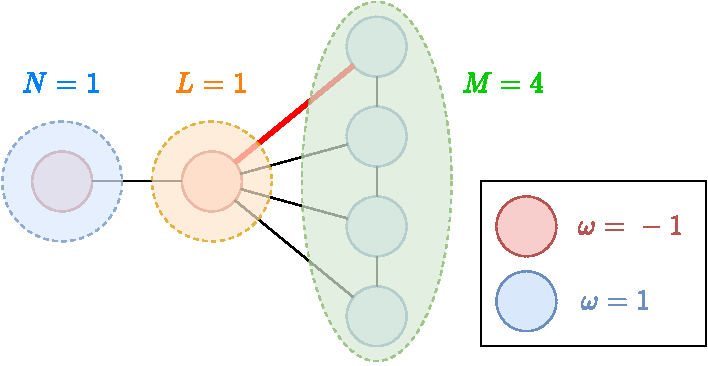
\includegraphics[width=105mm]{images/three-body-application.pdf}
    \centering
    \caption{6つの振動子から構成されるネットワーク.このネットワークは3つの集団に分割することができる.
    $\Omega_M$は実効振動数$\omega_M=1$,サイズ$M=4$の集団で,$\Omega_L$は実効振動数$\omega_L=-1$,サイズ$L=1$の集団で,$\Omega_N$は実効振動数$\omega_N=-1$,サイズ$N=1$の集団である.}
    \label{fig:3body-application}
\end{figure}

このネットワークは3つの集団に分割することができる.
$\Omega_M$は実効振動数$\omega_M=1$,サイズ$M=4$の集団で,$\Omega_L$は実効振動数$\omega_L=-1$,サイズ$L=1$の集団で,$\Omega_N$は実効振動数$\omega_N=-1$,サイズ$N=1$の集団である.

この集団では$|\Omega|=2\gg|\omega|=0$より臨界結合強度を求めることができる.
式\eqref{eq:phase-diff-general}におけるパラメータは$a=4,\ \tilde{M}=4,\ \tilde{N}=1$であるから,
$K_1=0,\ K_2\sim 0.25,\ K_3\sim 0.3,\ K_4=4/3$である.
よって,式\eqref{eq:phase-diff-general}で結合強度をスケーリングしたことに注意して,図\ref{fig:cutting_N6K1}の結合強度$K=L\tilde{K}/n$が
\begin{equation*}
    0\leq \tilde{K}\lesssim 0.25
\end{equation*}
を満たすとき,$\Omega_L$及び$\Omega_N$のみが同期し,
\begin{equation*}
    0.25\lesssim \tilde{K}\lesssim 0.3
\end{equation*}
のとき,3つの集団のうちどの2つも同期しない.
そして,
\begin{equation*}
    0.3\lesssim \tilde{K}<\frac{4}{3}
\end{equation*}
を満たすとき,$\Omega_L$及び$\Omega_M$のみが同期し,
\begin{equation*}
    \tilde{K}\geq \frac{4}{3}
\end{equation*}
のとき,3つの集団全てが同期する.
このように結合強度に応じて大きく同期状態が変化する.

続いて,図\ref{fig:3body-application}において赤で示した枝を省いたときの同期状態の変化について述べる.
このとき,$a=3$となるため,
\begin{equation*}
    K_3<K_2\sim 0.47
\end{equation*}
である.
よって,$0.25\lesssim \tilde{K}\lesssim 0.33$のとき赤で示した枝を削除すると,3つの集団のうちどの2つも同期しない状態から,$\Omega_L$及び$\Omega_N$のみが同期する状態へ変化する.
そして,$0.33\lesssim \tilde{K}\lesssim 0.47$のとき赤で示した枝を削除すると,$\Omega_L$及び$\Omega_M$のみが同期する状態から,$\Omega_L$及び$\Omega_N$のみが同期する状態へ変化する.

このように,3体系の解析を用いると,2つの集団で近似できる系よりもより複雑なふるまいを示す系について同期状態を調べることが可能である.


\section{議論}
\label{sec:3body-discussion}
\subsection{同期状態の変化パターン}
\ref{sec:3body-critical}節では結合強度$K_1,\ K_2$については$|\Omega|\gg|\omega|$の場合について求めた.
また,\ref{sec:3body-summary}節では,$|\Omega|\gg|\omega|$の場合について,結合強度$K$の変化に対応する同期状態の変化パターンとその結合強度比$a$への依存性を調べた.

$a$を固定したときの変化パターンは,ネットワークの枝の本数を固定した場合の同期パターンに対応する.
変化パターンの$a$依存性を理解することで,既存の同期状態が分かっているネットワークに枝を追加・削除したときにどう同期状態が変化するか理解することができる.
よって,$a$を固定したときの変化パターンは枝の本数と同期状態の関係において重要な解析対象である.
したがって,他のパラメータ領域でも同様に同期状態の変化パターンの$a$依存性を調べることが期待される.

$|\Omega|\sim|\omega|$の場合,式\eqref{eq:3body-matome}の$K_1$は正しくない.
しかしながら,\ref{sec:3body-k3}節の議論と同様にして,固有振動数の近い振動子との同期の十分条件,つまり$K_1$の上界が与えられる.
\begin{equation}
    \label{K1-approx-dash}
    K_1\lessapprox\frac{|\omega|}{2-a}\coloneqq K'_1.
\end{equation}
このとき,$K'_1,\ K'_3,\ K_{41},\ K_{42}$は$a^\ast_1$で一致する.
すなわち,2体が同期する場合鞍替えは起こらず,結合強度$K$を大きくしても3体の同期が起こるということになるため,これまでの議論と反する.
よって,$K'_1,\ K'_3$を用いて同期状態の変化パターンを議論するのは不適切である.
よって,一般のパラメータ領域での同期状態の変化パターンを解析する上では,$K_1,\ K_3$について$K'_1,\ K'_3$のような上界ではなくより正しい値を求めることが必要になると思われる.

$|\Omega|\sim|\omega|$の分岐図を図\ref{fig:3body-phase-boundary}に示す.
結合強度比$a$を大きくすると,図\ref{fig:3body-notapprox150}のような同期状態の変化パターンから,図\ref{fig:3body-notapprox175},図\ref{fig:3body-notapprox200}の順に変化パターンが変化することがわかる.
そして,3体がどれも非同期の状態から3体が同期するような図\ref{fig:3body-symmetry}のような状況は起きえないことがわかる.

また,他のパラメータに対し同様に数値実験を行った結果から,3体がどれも非同期の状態から3体が同期する必要十分条件が$\Omega=\pm\omega$であり,多くのパラメータ領域では起きえないことが推測される.
異なる振動数をもつ集団が同時に同じ振動数に変化することがほとんどのパラメータ領域では起きえないとすれば,異なる振動子の集団がほとんどの場合2つしか同時に同じ振動数に変化することはないと考えることができる.
よって,平均場近似 (式\eqref{eq:3body-default}) の仮定が成り立ち続けるような枝の増減に伴うネットワークの同期状態の変化を調べる場合,ネットワークを最も簡略化された3体系に分割して解析することが有用となる.

\begin{figure}[tbp]
\centering
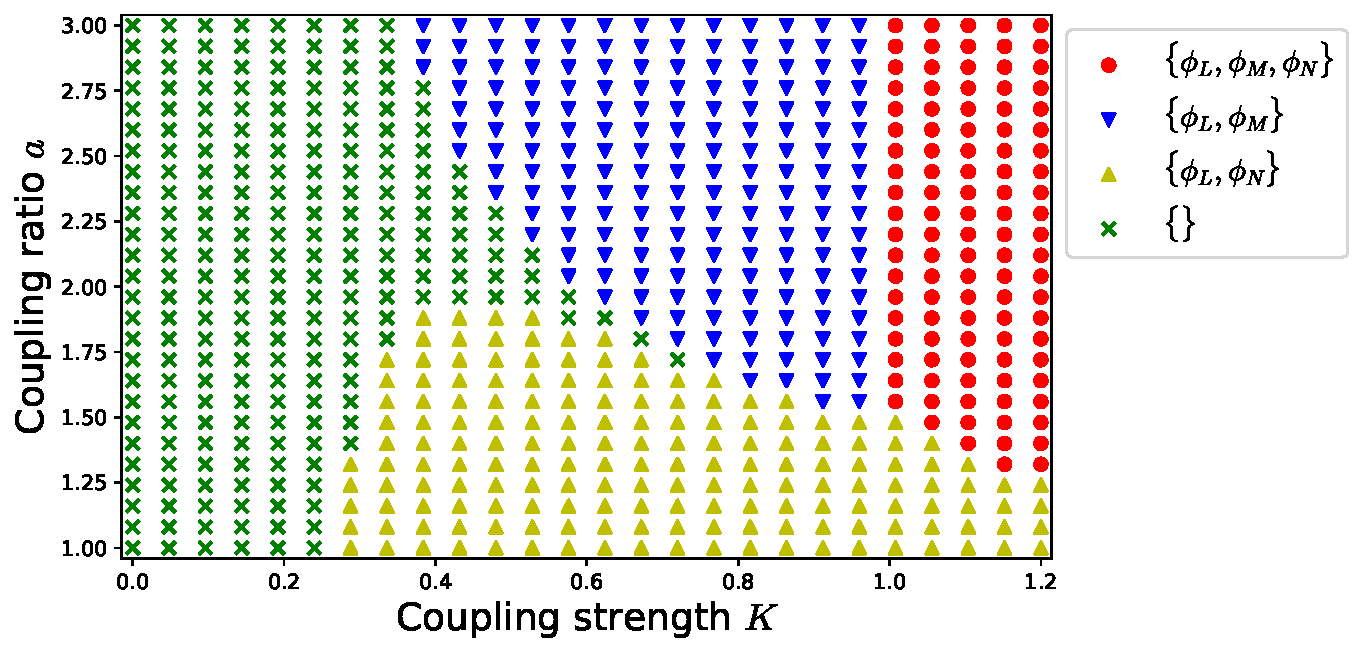
\includegraphics[width=135mm]{./images/three-body-phase-boundary.pdf}
\centering
\caption{$\Omega=-2,\ \omega=0.5$のときの結合強度$K$,結合強度$a$における3体系の同期状態を表す分岐図.
各格子点に対し,3体全体の同期・固有振動数の離れた振動子との同期・固有振動数の近い振動子との同期・3体とも非同期の4状態を示している.\\
$a=1.5,\ 1.8$を境に$a$を固定し$K$を変化させたときの同期状態の変化パターンが変化している.}
\label{fig:3body-phase-boundary}
\end{figure}

\subsection{$|\Omega|\gg|\omega|$を用いて求めた臨界結合強度の適用限界}
\ref{sec:3body-critical}節において$\varepsilon=|\Omega|/|\omega|\ll 1$を仮定し求めた結合強度$K_1,\ K_2$について,どの程度の$\varepsilon$まで有効か調べる.
ここでは,\ref{sec:3body-k12}節において求めた$K_2$の閉形式の表現である式\eqref{eq:K2-approx}だけでなく,式\eqref{eq:nit-H1},\ \eqref{eq:nit-H2}より定まる以下のような$y$の近恒等変換$z$の微分方程式を考える.
\begin{equation}
    \label{eq:k1k2-open}
    \dot{z}=\varepsilon+kH_1(z)+k^2H_2(z)+O(k^3,\varepsilon^2)
\end{equation}
この式が$\dot{z}=0$の解を持つ同期条件を以下では開形式の同期条件と呼ぶことにする.
特に,開形式の同期条件から定まる臨界結合強度を開形式の臨界結合強度と略することとする.
開形式の同期条件の境界は$K$-$a$平面上の連結な曲線であり,ある結合強度比$a$に対して2つの交点を持つ.
開形式の同期条件は振動数の近い振動子が同期する条件であるため,2つの交点は$K_1,\ K_2$に対応すると考えられる.

まず,$a=1$のときの$K_1$について数値実験による値と閉形式の値(式\eqref{eq:K1-approx})と開形式の同期条件から定まる値を様々な$\varepsilon$で比較したものを図\ref{fig:k1-compare}に示す.
$\varepsilon$が大きくなると閉形式やや外れているものの,$\varepsilon=0.3$までは閉形式,開形式ともにいい精度で近似できている.

\begin{figure}[tbp]
\centering
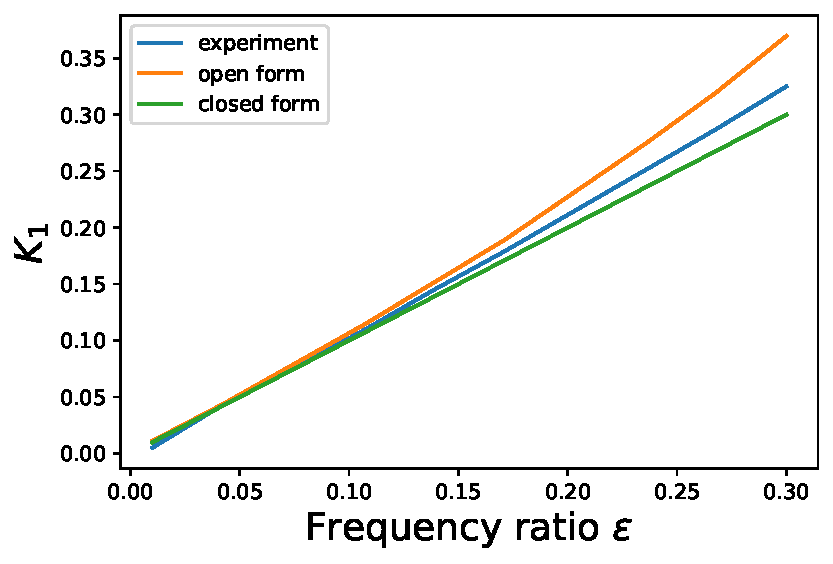
\includegraphics[width=105mm]{./images/k1-compare.pdf}
\centering
\caption{$a=1$のときの$K_1$について数値実験による値と閉形式の値(式\eqref{eq:K1-approx})と開形式の同期条件から定まる値を様々な$\varepsilon$で比較した.
$\varepsilon$が大きくなると閉形式やや外れているものの,$\varepsilon=0.3$までは閉形式,開形式ともにいい精度で近似できている.}
\label{fig:k1-compare}
\end{figure}

次に,$a=1,\ 1.7$のときの$K_1$について閉形式の値及び開形式の同期条件から定まる値の数値実験による値との誤差を様々な$\varepsilon$で比較したものを図\ref{fig:k1-error}に示す.
閉形式の値において$\varepsilon$の増加に伴った誤差の拡大が$a=1$より$a=1.7$で大きい.
これは,図\ref{fig:3body-phase}で$a$が大きいほど$K_1$の真の値が大きいが,式\eqref{eq:K1-approx}は定数であるため,$a$が大きいほど誤差が拡大していると考えられる.
一方,開形式については閉形式に比べ誤差及び$a$の増大に伴う誤差の増大は小さくなっている.

\begin{figure}[tbp]
\centering
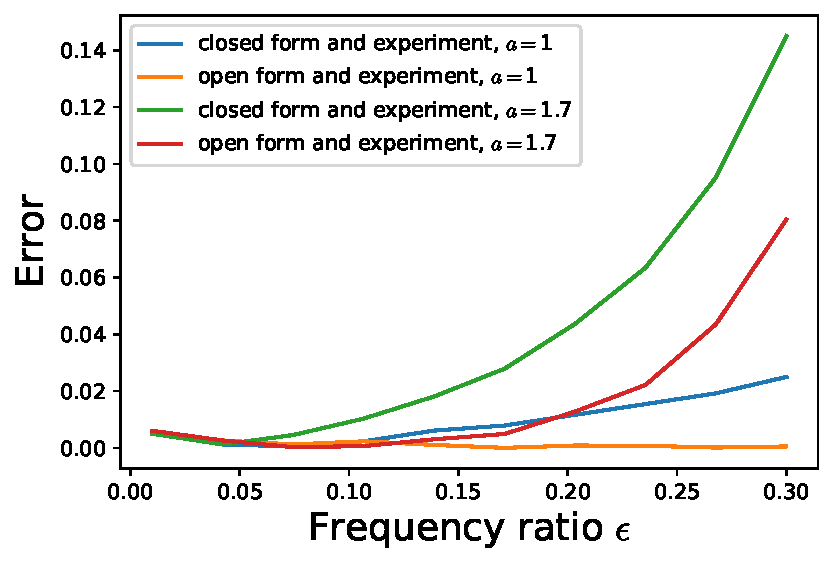
\includegraphics[width=105mm]{./images/k1-error.pdf}
\centering
\caption{$a=1,\ 1.7$のときの$K_1$について数値実験による値と閉形式の値と開形式の同期条件から定まる値を様々な$\varepsilon$で比較した.
閉形式の値において$\varepsilon$の増加に伴った誤差の拡大が$a=1$より$a=1.7$で大きい一方で,開形式については閉形式に比べ誤差及び$a$の増大に伴う誤差の増大は小さくなっている.}
\label{fig:k1-error}
\end{figure}

$a=4$のときの$K_2$について数値実験による値と閉形式の値(式\eqref{eq:K2-approx})と開形式の同期条件から定まる値を様々な$\varepsilon$で比較したものを図\ref{fig:k2-compare}に示す.
$K_1$と比べると,閉形式.開形式ともに精度が落ちるものの.$\varepsilon=0.045$までは閉形式,開形式ともにある程度の精度で近似できている.
ここで,開形式よりも,より多くの仮定を課した閉形式が数値実験による値に近いのは,閉形式において$|\varepsilon k|\ll 1,\ |a\varepsilon k^2| \ll 1$という$\varepsilon$や$k$だけでなく$a$にも依存した仮定を課していることによるアーチファクトであると考えられる.

\begin{figure}[tbp]
\centering
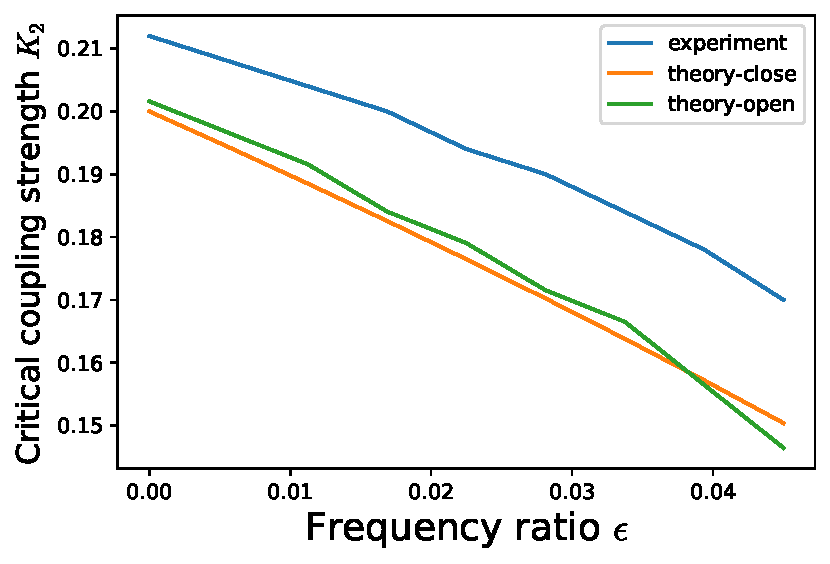
\includegraphics[width=105mm]{./images/k2-compare.pdf}
\centering
\caption{$a=5$のときの$K_2$について数値実験による値と閉形式の値(式\eqref{eq:K1-approx})と開形式の同期条件から定まる値を様々な$\varepsilon$で比較した.
$K_1$と比べると,閉形式.開形式ともに精度が落ちるものの.$\varepsilon=0.045$までは閉形式,開形式ともにある程度の精度で近似できている.}
\label{fig:k2-compare}
\end{figure}

図\ref{fig:3body-phase},\ref{fig:3body-phase-boundary}からわかるように,$K_1$及び$K_2$はある$(K,a)$で一致し,$K$-$a$平面で連結な曲線を構成する.
開形式による$K_1$及び$K_2$も連結な曲線となるため,ある$a$における両曲線の値を異なる$\varepsilon$で比較し精度を評価することが考えられる.
$a=5$のときの$K_1,\ K_2$について数値実験による値とと開形式の同期条件から定まる値を様々な$\varepsilon$で比較したものを図\ref{fig:k1k2-compare}に示す.
$K_1$よりも$K_2$で開形式の精度が悪い.
また,$K_1$と$K_2$が一致する$\varepsilon$も数値実験の値と開形式の値とで異なる.
よって,開形式の値は,閉形式の値を用いるよりも$a$依存性をより精度よく近似しているものの,$\varepsilon$が大きくなると有効ではないと考えられる.

\begin{figure}[tbp]
\centering
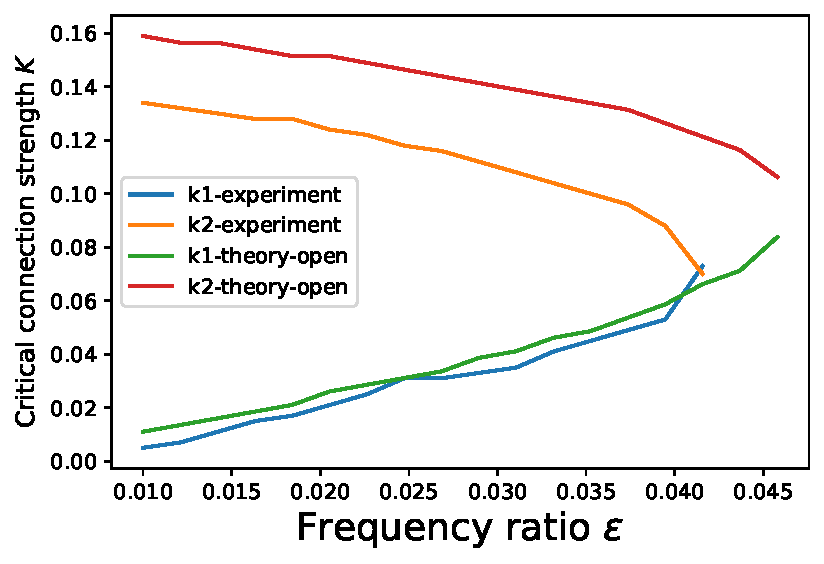
\includegraphics[width=105mm]{./images/k1k2-compare-open.pdf}
\centering
\caption{$a=4$のときの$K_1,\ K_2$について数値実験による値と閉形式の値(式\eqref{eq:K1-approx})と開形式の同期条件から定まる値を様々な$\varepsilon$で比較した.
$K_1$よりも$K_2$で開形式の精度が悪い.
また,$K_1$と$K_2$が一致する$\varepsilon$も数値実験の値と開形式の値とで異なる.}
\label{fig:k1k2-compare}
\end{figure}

以上より,\ref{sec:3body-critical}節で求めた閉形式の臨界結合強度は$\varepsilon$が極めて小さい場合は有効であるが,$\varepsilon\sim 1$のような場合は有効ではない.
また,開形式の臨界結合強度は$K_1$及び$K_2$を連結な曲線で表現するという閉形式の臨界結合強度が持たない性質を持っているものの,
$\varepsilon$が大きい領域での近似誤差は依然として大きい.
このため,$\varepsilon\sim 1$の場合の性質を調べるためには,$\varepsilon\ll 1$を利用せずに臨界結合強度を求めることが期待される.

\subsection{3体系の適用範囲}
\label{sec:3body-application}
\ref{fig:switch}節では,以下のような手順で3体系を導入した.
\begin{itemize}
    \item ある連結な部分ネットワークにおいて部分ネットワークに属する振動子間に枝が追加されることを考える.
    \item 加えられた枝の端点が異なる集団に属する形で,3つの同期した集団が鎖状に繋がるように分割する.このとき,集団間の枝を無視した状態で各集団が同期することを仮定する.
    また,鎖状に繋がった3つの集団のうち両端の集団の間の枝は無視できるほど少ないことを仮定する.
    \item 各集団をそれぞれ平均場近似を行い,集団間の枝の数に応じた結合強度で結合しているみなす.
\end{itemize}
ここで,必ずしも3つの集団が存在する必要はない.
2つの集団に分割可能であれば,集団間の枝を無視した状態でそれぞれの集団を平均場近似を行うことで2体の同期問題に帰着することができる.
このように,3体系を適用できる状況であっても適用する必要がない場合がある.

しかしながら,以下のような場合は3体系を用いて同期状態を求めることができないと考えられる.
\renewcommand{\labelenumi}{Case \theenumi}
\begin{enumerate}
    \item \label{counter-case1} 
    どのように分割しても異なる実行振動数の集団が必ず4つ以上存在する場合.
    \item \label{counter-case2}
    異なる実行振動数の集団が3つ以内になるように分割できるものの,どのように分割しても,鎖状に連なった3つの集団において両端の集団間の枝がそれ以外の集団間の枝に比べ無視できない場合.
    \item \label{counter-case3}
    注目する枝を除いた場合は3つの集団に分割できるものの,そのどのような分割に対しても,注目する枝を加えると4つ以上の集団に分かれてしまう場合.
\end{enumerate}

Case \ref{counter-case1}, Case \ref{counter-case2} に該当する部分ネットワークの存在は明らかであるが,Case \ref{counter-case3} は明らかではない.
3つの集団に分かれたものに枝を加えると4つの集団に分かれる場合に存在すれば十分である.
特に,3つの集団のうち1つの集団が他の集団と弱く結合していると仮定する.
このとき,2つの集団に対して枝を増やしたときに3つの集団に分かれる場合があることを示せばいい.
実効振動数が近い2つの集団が同期した状態で,実効振動数が離れた集団との間の枝を追加すると,結合強度比$a$が増加し,3つ全てが非同期となる場合がある.
実際,$K$-$a$平面における同期状態図(図\ref{fig:3body-phase-m5})において,$a=m/n$及び$a=(m+1)/n$の直線の間に$K_1,\ K_2$に対応する曲線を含むような枝の本数の組$(m,n)$が,各$K$に対して存在する.

\begin{figure}[tbp]
    \centering
    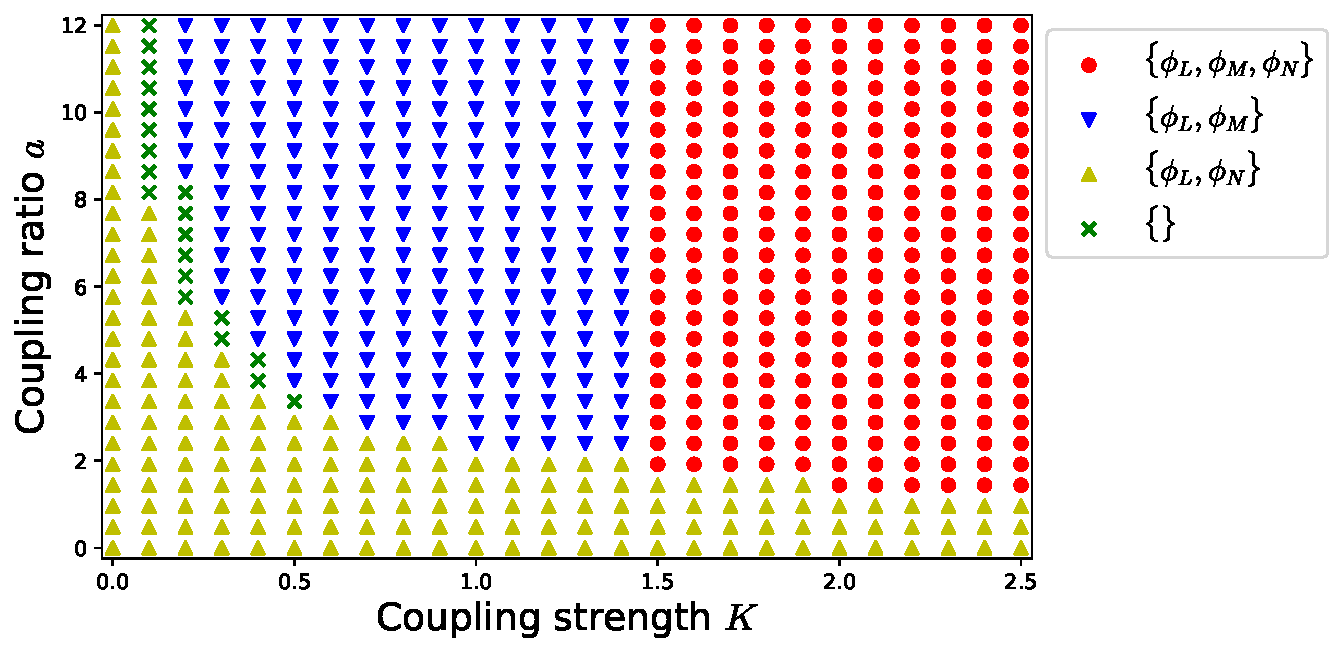
\includegraphics[width=135mm]{./images/three-body-phase-m5.pdf}
    \centering
    \caption{$\Omega=-2,\ \omega=0,\ M=5,\ N=1$のときの結合強度$K$,\ 結合強度比$a$における同期状態図.\\
    $m=3$から$m=4$に枝を増やすと$n=1$であるので$a=3$から$a=4$へ変化し,2つが同期していた状態から3つが非同期な状態へ同期状態が変化する.}
    \label{fig:3body-phase-m5}
\end{figure}

% \subsection{3体系における実行振動数の偏り}
% この3体系のモデルは様々な振動子ネットワークの同期状態の解析に利用することができるが,
% 用いる振動子ネットワークの構造及び振動数分布によって,3体の実効振動数は変化すると考えられる.

% 本研究で用いたERモデルにおいても,定性的な議論が考えられる.
% ERモデルでは,\ref{sec:er-graph}節で述べたように,枝の数がある一定増大すると巨大な連結成分が出現し,多くの頂点はその連結成分に属する.
% このため,ERモデルのネットワークに対して3体系が適用できる場合,巨大な連結成分を含んだ部分ネットワークであることが多い.
% そこで,巨大な連結成分を含んだネットワークにおいて鞍替えが起こる以下の場合について実行振動数の分布を考える.
% 巨大な連結成分に含まれるサイズの大きな集団$\Omega_M$と同期していた集団$\Omega$が,巨大な連結成分に含まれない集団$\Omega_N$と枝が繋がることによって誘引され分離もしくは鞍替えが起こる.
% このとき,\ref{sec:3body-general}で述べたように,枝を追加する前に属していた集団$\Omega_M$の実行振動数$\omega_M$が集団$\Omega$の実行振動数$\omega$に近いほど分離及び鞍替えが起こりやすい.
% そして,追加した後に属する集団$\Omega_N$の実行振動数$\omega_N$が$\omega$に近く,$\Omega$との間の枝が多いほど鞍替えが起こりやすい.
% 枝を新たに1本だけ追加する場合を考えると,枝を増やす前は$\Omega$は$\Omega_M$と同期していたことから$\Omega_N$,$\Omega$間の枝は多くない.
% よって,多くの場合で$\Omega\gg\omega$となると考えられる.
\end{document}